\section{Inbetriebnahme}

\subsection{Grundlagen}

\subsubsection{Anlagenübersicht}

\begin{figure}[H]
   \centering
   \fbox{\includegraphics[width=0.8\textwidth]{Bilder/1. Grundlagen/(1.1) Anlagenübersicht.png}}
   \caption[Anlagenübersicht]{Anlagenübersicht}
   \label{fig:Bild1.1}
\end{figure}

\begin{figure}[H]
   \centering
   \fbox{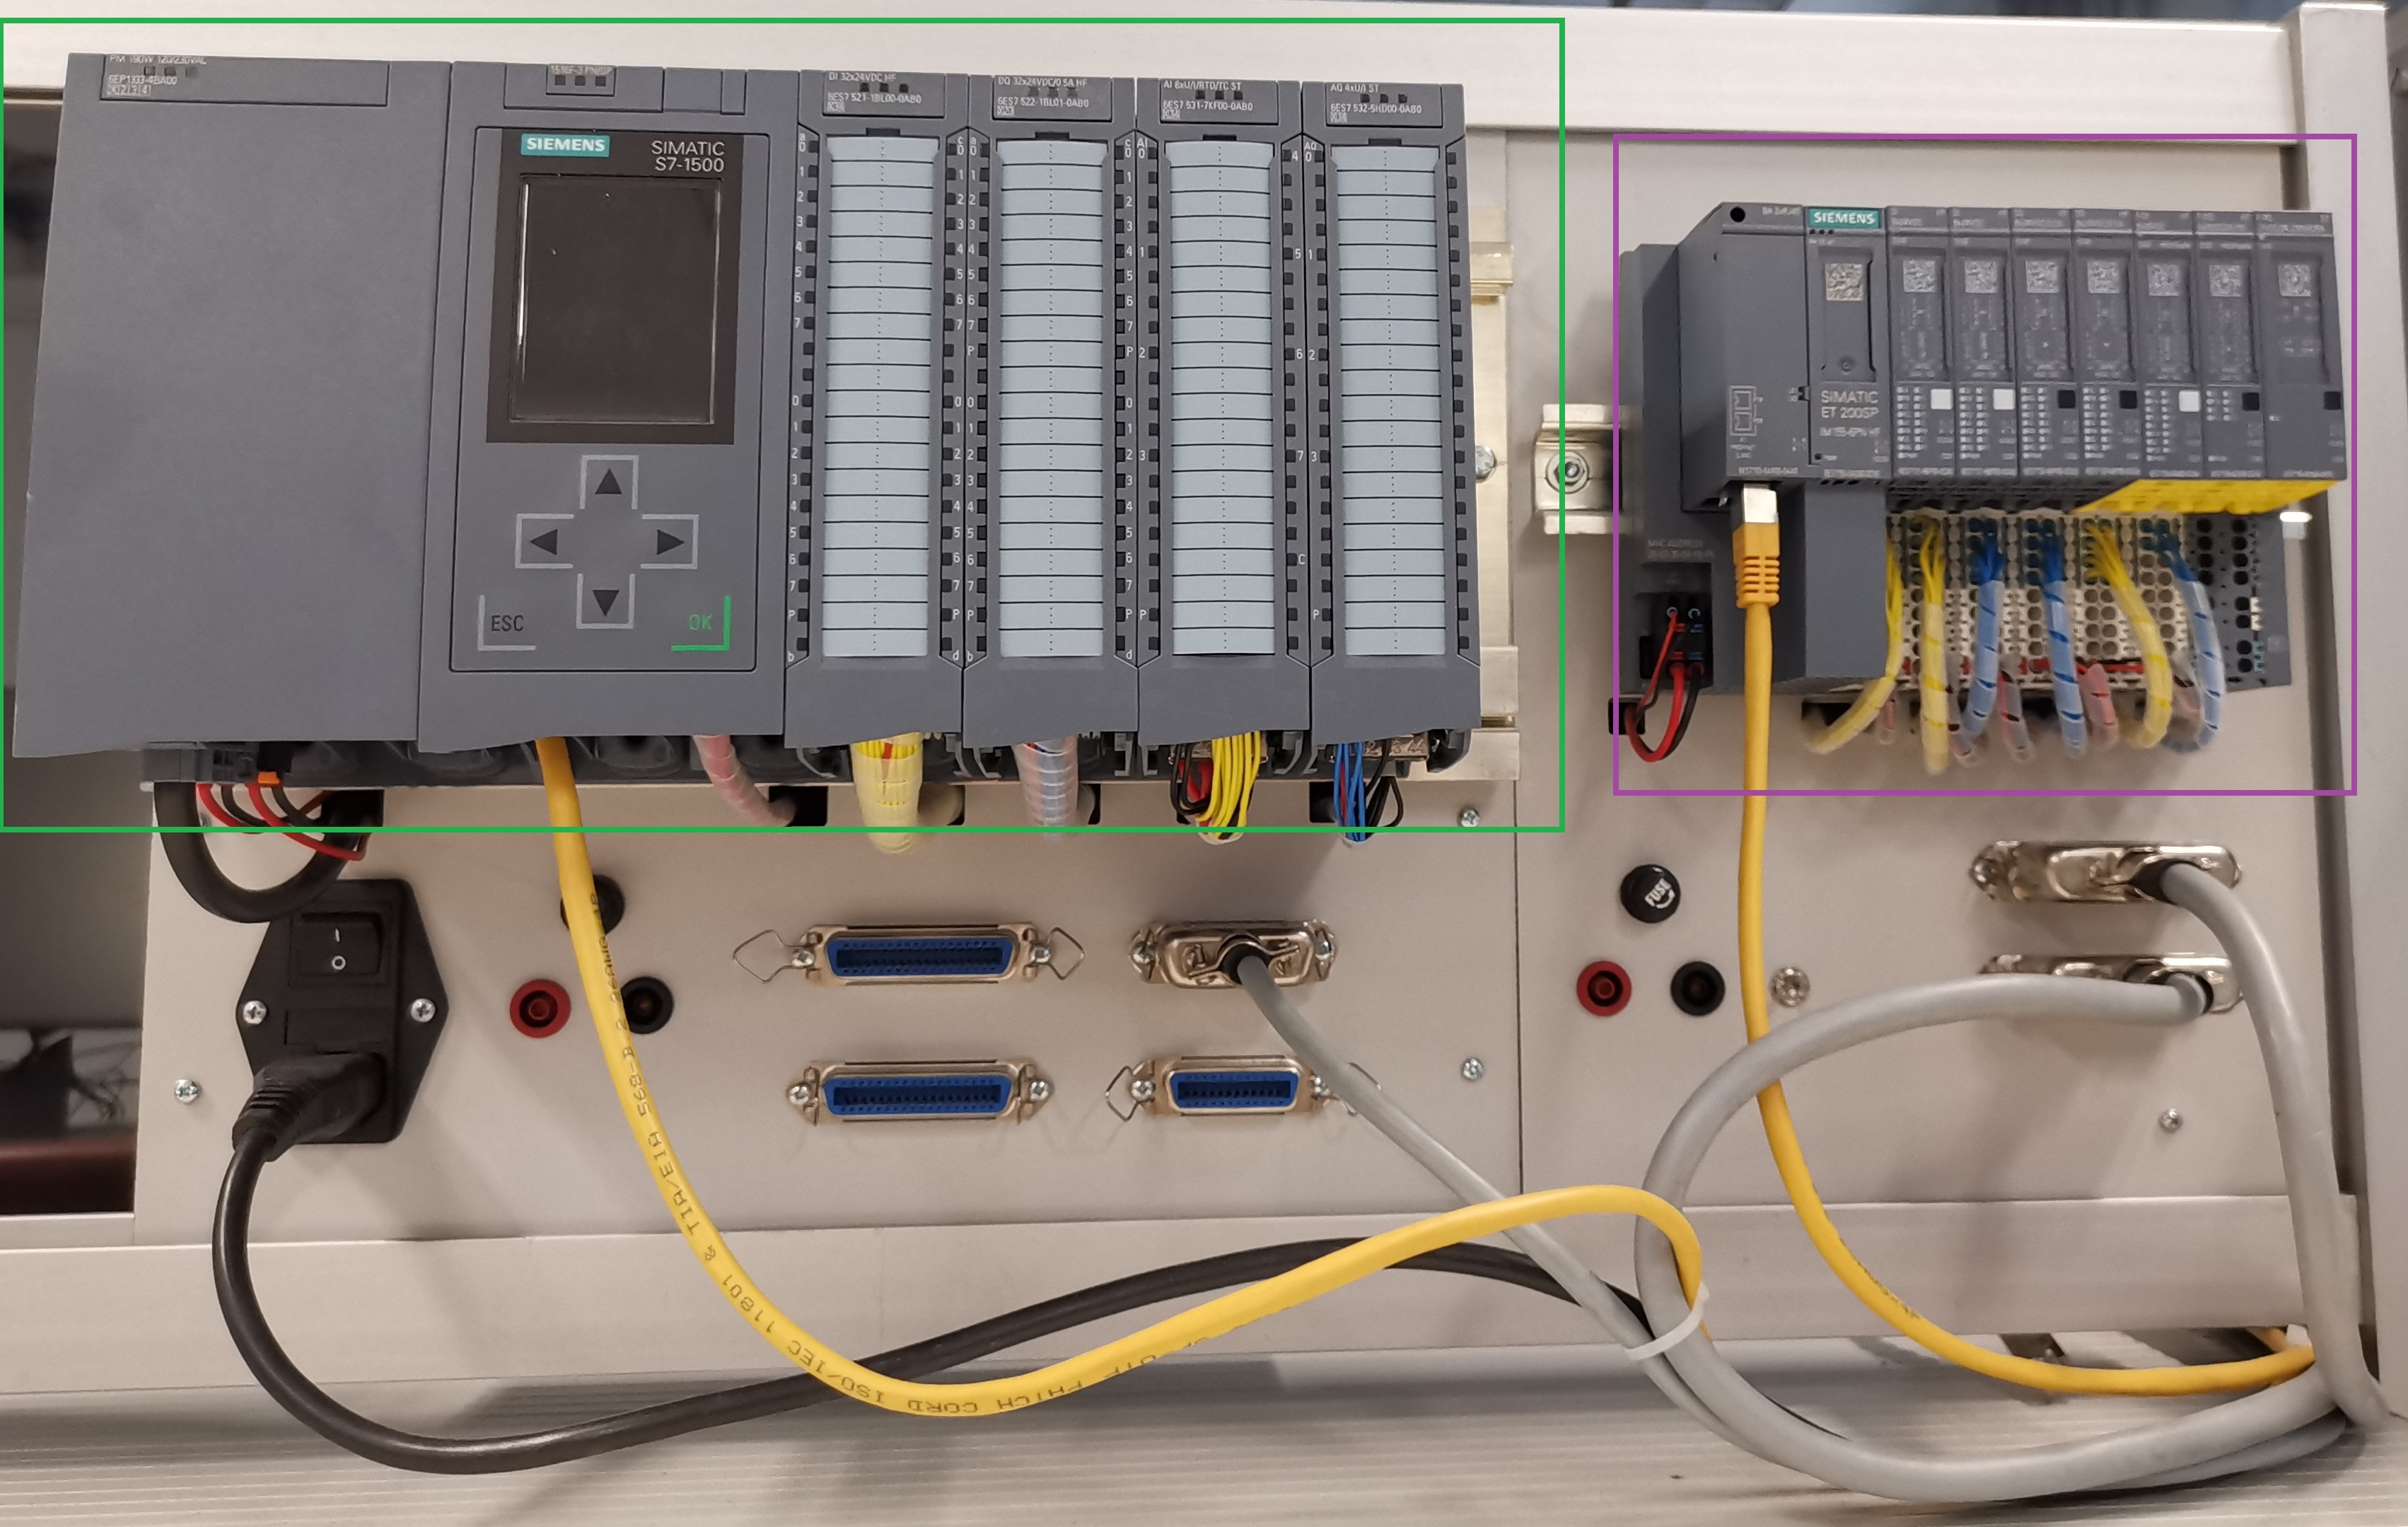
\includegraphics[width=0.8\textwidth]{Bilder/1. Grundlagen/(1.2) Reale Anlage.jpg}}
   \caption[Reale Anlage]{Reale Anlage (links: S7-1500; rechts: ET 200SP)}
   \label{fig:Bild1.2}
\end{figure}

\subsubsection{PROFINET-Gerätenamen und IP-Adressen im Raum WH G-420}
\begin{figure}[H]
    \centering
    \begin{tikzpicture}[framed][domain=0:0]
        % Umrandung zeichnen
        \draw[black, very thick] (0,0) rectangle (15,17);
        
        % Eingangstür zeichnen
        \draw[black, very thick](15,0.7) -- (13, 0.7);
        \draw[grey, very thin] (15,2.7) arc (90:180:2);
        
        % Tür zum Büro
        \draw[black, very thick](9, 17) -- (9, 15);
        \draw[grey, very thin] (11, 17) arc (0:-90:2);
        
        % Tafel
        \draw[black, fill = black] (5.5, 0.3) rectangle (9.5, 0.4);
        \draw[black, fill = black] (9.5,0.3) -- (11.5, 1) -- ++(109.29:0.1cm) -- ++(199.29:2.12cm) -- ++(289.29:0.1cm);
        \draw[black, fill = black] (5.5, 0.3) -- (3.5, 1) -- ++(70.71:0.1cm) -- ++(-19.29:2.12cm) -- ++(-109.29:0.1cm);
        
        % Arbeitsplätze Wand
        \draw[black, dashed] (11.3, 2.9) rectangle (14.8, 5.7);
        \draw[black, dashed] (11.3, 5.9) rectangle (14.8, 8.7);
        \draw[black, dashed] (11.3, 8.9) rectangle (14.8, 11.7);
        \draw[black, dashed] (11.3, 11.9) rectangle (14.8, 14.7);
        
        % Arbeitsplätze Fenster
        \draw[black, dashed] (0.2, 2.9) rectangle (3.7, 5.7);
        \draw[black, dashed] (0.2, 5.9) rectangle (3.7, 8.7);
        \draw[black, dashed] (0.2, 8.9) rectangle (3.7, 11.7);
        \draw[black, dashed] (0.2, 11.9) rectangle (3.7, 14.7);
        
        % Arbeitsplätze Gang
        \draw[black, dashed] (3.9, 2.9) rectangle (7.4, 5.7);
        \draw[black, dashed] (3.9, 5.9) rectangle (7.4, 8.7);
        \draw[black, dashed] (3.9, 8.9) rectangle (7.4, 11.7);
        \draw[black, dashed] (3.9, 11.9) rectangle (7.4, 14.7);
        
        % Raum
        \node[font=\bfseries, scale = 1] at (2, 16.5) {Raum WH G-420};
        
        % Subnetz-Text
        \node[scale = 0.8] at (1.9, 16) {Subnetz: 255.255.255.0};
        
        % Gerätenamen PC's & IP-Adressen Fenster
        \node[font=\bfseries, scale = 0.8] at (1.85, 14.4) {FB1-G420-04};
        \node[scale = 0.75] at (1.85, 14) {192.168.1.14};
        \node[font=\bfseries, scale = 0.8] at (1.85, 13.5) {s7-1500-fenster-4};
        \node[scale = 0.75] at (1.85, 13.1) {192.168.1.114};
        \node[font=\bfseries, scale = 0.8] at (1.85, 12.6) {et-200-fenster-4};
        \node[scale = 0.75] at (1.85, 12.2) {192.168.1.134};
        
        \node[font=\bfseries, scale = 0.8] at (1.85, 11.4) {FB1-G420-03};
        \node[scale = 0.75] at (1.85, 11) {192.168.1.13};
        \node[font=\bfseries, scale = 0.8] at (1.85, 10.5) {s7-1500-fenster-3};
        \node[scale = 0.75] at (1.85, 10.1) {192.168.1.113};
        \node[font=\bfseries, scale = 0.8] at (1.85, 9.6) {et-200-fenster-3};
        \node[scale = 0.75] at (1.85, 9.2) {192.168.1.133};
        
        \node[font=\bfseries, scale = 0.8] at (1.85, 8.4) {FB1-G420-02};
        \node[scale = 0.75] at (1.85, 8) {192.168.1.12};
        \node[font=\bfseries, scale = 0.8] at (1.85, 7.5) {s7-1500-fenster-2};
        \node[scale = 0.75] at (1.85, 7.1) {192.168.1.112};
        \node[font=\bfseries, scale = 0.8] at (1.85, 6.6) {et-200-fenster-2};
        \node[scale = 0.75] at (1.85, 6.2) {192.168.1.132};
        
        \node[font=\bfseries, scale = 0.8] at (1.85, 5.4) {FB1-G420-01};
        \node[scale = 0.75] at (1.85, 5) {192.168.1.11};
        \node[font=\bfseries, scale = 0.8] at (1.85, 4.5) {s7-1500-fenster-1};
        \node[scale = 0.75] at (1.85, 4.1) {192.168.1.111};
        \node[font=\bfseries, scale = 0.8] at (1.85, 3.6) {et-200-fenster-1};
        \node[scale = 0.75] at (1.85, 3.2) {192.168.1.131};
        
        % Gerätenamen PC's & IP-Adressen Gang
        \node[font=\bfseries, scale = 0.8] at (5.6, 14.4) {FB1-G420-08};
        \node[scale = 0.75] at (5.6, 14) {192.168.1.18};
        \node[font=\bfseries, scale = 0.8] at (5.6, 13.5) {s7-1500-gang-4};
        \node[scale = 0.75] at (5.6, 13.1) {192.168.1.118};
        \node[font=\bfseries, scale = 0.8] at (5.6, 12.6) {et-200-gang-4};
        \node[scale = 0.75] at (5.6, 12.2) {192.168.1.138};
        
        \node[font=\bfseries, scale = 0.8] at (5.6, 11.4) {FB1-G420-07};
        \node[scale = 0.75] at (5.6, 11) {192.168.1.17};
        \node[font=\bfseries, scale = 0.8] at (5.6, 10.5) {s7-1500-gang-3};
        \node[scale = 0.75] at (5.6, 10.1) {192.168.1.117};
        \node[font=\bfseries, scale = 0.8] at (5.6, 9.6) {et-200-gang-3};
        \node[scale = 0.75] at (5.6, 9.2) {192.168.1.137};
        
        \node[font=\bfseries, scale = 0.8] at (5.6, 8.4) {FB1-G420-06};
        \node[scale = 0.75] at (5.6, 8) {192.168.1.16};
        \node[font=\bfseries, scale = 0.8] at (5.6, 7.5) {s7-1500-gang-2};
        \node[scale = 0.75] at (5.6, 7.1) {192.168.1.116};
        \node[font=\bfseries, scale = 0.8] at (5.6, 6.6) {et-200-gang-2};
        \node[scale = 0.75] at (5.6, 6.2) {192.168.1.136};
        
        \node[font=\bfseries, scale = 0.8] at (5.6, 5.4) {FB1-G420-05};
        \node[scale = 0.75] at (5.6, 5) {192.168.1.15};
        \node[font=\bfseries, scale = 0.8] at (5.6, 4.5) {s7-1500-gang-1};
        \node[scale = 0.75] at (5.6, 4.1) {192.168.1.115};
        \node[font=\bfseries, scale = 0.8] at (5.6, 3.6) {et-200-gang-1};
        \node[scale = 0.75] at (5.6, 3.2) {192.168.1.135};
        
        % Gerätenamen PC's & IP-Adressen Wand
        \node[font=\bfseries, scale = 0.8] at (13, 14.4) {FB1-G420-12};
        \node[scale = 0.75] at (13, 14) {192.168.1.22};
        \node[font=\bfseries, scale = 0.8] at (13, 13.5) {s7-1500-wand-4};
        \node[scale = 0.75] at (13, 13.1) {192.168.1.122};
        \node[font=\bfseries, scale = 0.8] at (13, 12.6) {et-200-wand-4};
        \node[scale = 0.75] at (13, 12.2) {192.168.1.142};
        
        \node[font=\bfseries, scale = 0.8] at (13, 11.4) {FB1-G420-11};
        \node[scale = 0.75] at (13, 11) {192.168.1.21};
        \node[font=\bfseries, scale = 0.8] at (13, 10.5) {s7-1500-wand-3};
        \node[scale = 0.75] at (13, 10.1) {192.168.1.121};
        \node[font=\bfseries, scale = 0.8] at (13, 9.6) {et-200-wand-3};
        \node[scale = 0.75] at (13, 9.2) {192.168.1.141};
        
        \node[font=\bfseries, scale = 0.8] at (13, 8.4) {FB1-G420-10};
        \node[scale = 0.75] at (13, 8) {192.168.1.20};
        \node[font=\bfseries, scale = 0.8] at (13, 7.5) {s7-1500-wand-2};
        \node[scale = 0.75] at (13, 7.1) {192.168.1.120};
        \node[font=\bfseries, scale = 0.8] at (13, 6.6) {et-200-wand-2};
        \node[scale = 0.75] at (13, 6.2) {192.168.1.140};
        
        \node[font=\bfseries, scale = 0.8] at (13, 5.4) {FB1-G420-09};
        \node[scale = 0.75] at (13, 5) {192.168.1.19};
        \node[font=\bfseries, scale = 0.8] at (13, 4.5) {s7-1500-wand-1};
        \node[scale = 0.75] at (13, 4.1) {192.168.1.119};
        \node[font=\bfseries, scale = 0.8] at (13, 3.6) {et-200-wand-1};
        \node[scale = 0.75] at (13, 3.2) {192.168.1.139};
    \end{tikzpicture}
    \caption[IP-Adressen und PROFINET-Gerätenamen im Raum WH G-420]{IP-Adressen und PROFINET-Gerätenamen im Raum WH G-420}
    \label{fig:Bild1.3}
\end{figure}

\subsection{Neues Projekt anlegen} \label{sec: Neues_Projekt_anlegen}

\subsubsection{TIA Portal öffnen}

Im PC-Menü \glqq\textbf{Start}\grqq\:nach dem \textbf{TIA Portal} suchen (hier Version: V17) und Software starten.
\begin{figure}[H]
   \centering
   \fbox{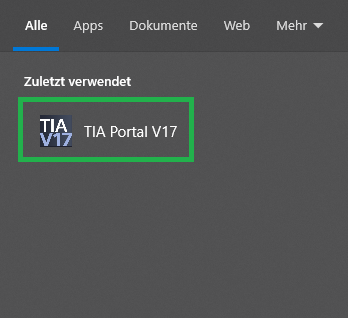
\includegraphics[width=0.4\textwidth]{Bilder/2. Neues Projekt anlegen/(2.1) TIA Portal V17 oeffnen.png}}
   \caption[TIA Portal öffnen]{TIA Portal öffnen}
   \label{fig:Bild2.1}
\end{figure}

\subsubsection{Projekt erstellen}

\textbf{Projektname, Pfad} und \textbf{Autor} des neuen Projektes vergeben und mit \glqq\textbf{Erstellen}\grqq\:bestätigen.
\begin{figure}[H]
   \centering
   \fbox{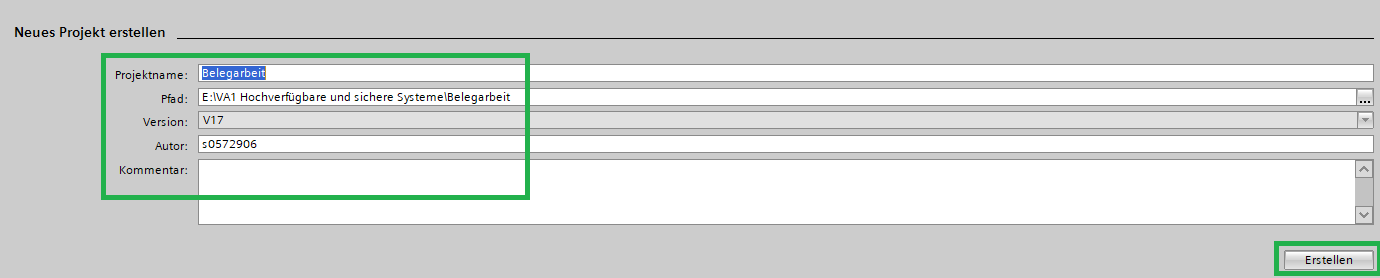
\includegraphics[width=1.0\textwidth]{Bilder/2. Neues Projekt anlegen/(2.2) Neues Projekt erstellen.png}}
   \caption[Neues Projekt erstellen]{Neues Projekt erstellen}
   \label{fig:Bild2.2}
\end{figure}

\clearpage

\subsubsection{Projektansicht öffnen}

Die Projektansicht über \glqq\textbf{Projektansicht öffnen}\grqq\:aufrufen und weitere Einstellungen vornehmen.
\begin{figure}[H]
   \centering
   \fbox{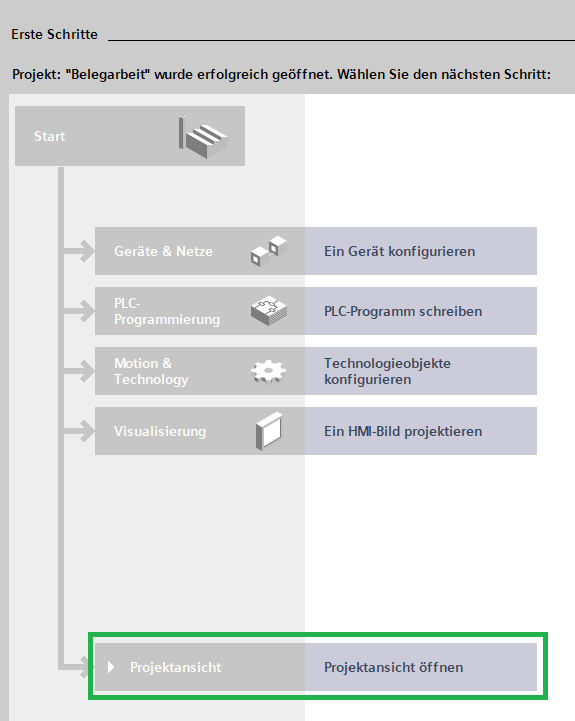
\includegraphics[width=0.6\textwidth]{Bilder/2. Neues Projekt anlegen/(2.3) Projektansicht oeffnen.png}}
   \caption[Projektansicht öffnen]{Projektansicht öffnen}
   \label{fig:Bild2.3}
\end{figure}

\subsection{Konfiguration der S7-1500} \label{sec: Konfiguration_der_S7_1500}

\subsubsection{S7-1500 hinzufügen}
Über \glqq\textbf{Neues Gerät hinzufügen}\grqq\:nach \textbf{6ES7 5XX-XXXXX-XXXX} suchen und mit \glqq\textbf{OK}\grqq\:bestätigen.\\
Pfad: Controller > SIMATIC S7-1500 > CPU > Nicht spezifizierte CPU 1500
\begin{figure}[H]
    \centering
   \begin{minipage}[b]{.4\linewidth}
        \centering
        \fbox{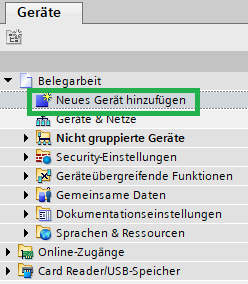
\includegraphics[width=1\linewidth]{Bilder/3. Konfiguration der S7-1500/3.1 S7-1500 hinzufügen/(3.1.1) Neues Geraet hinzufuegen.png}}
        \caption[Neues Gerät hinzufügen]{Neues Gerät hinzufügen}
        \label{fig:Bild3.1}
   \end{minipage}
   \hspace{.1\linewidth}% Abstand zwischen Bilder
   \begin{minipage}[b]{.4\linewidth}
        \centering
        \fbox{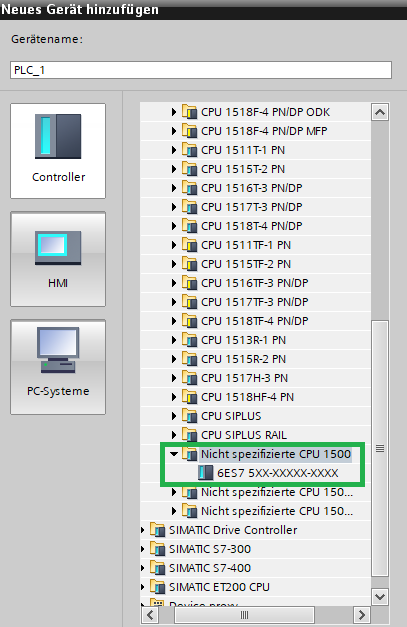
\includegraphics[width=1\linewidth]{Bilder/3. Konfiguration der S7-1500/3.1 S7-1500 hinzufügen/(3.1.2) SPS auswaehlen.png}}
        \caption[S7-1500 auswählen]{S7-1500 auswählen}
        \label{fig:Bild3.2}
   \end{minipage}
\end{figure}

\clearpage

\subsubsection{Kommunikation herstellen}
In der \textbf{Gerätesicht} der S7-1500 über \glqq\textbf{ermitteln}\grqq\:die entsprechende Hardware suchen.
\begin{figure}[H]
   \centering
   \fbox{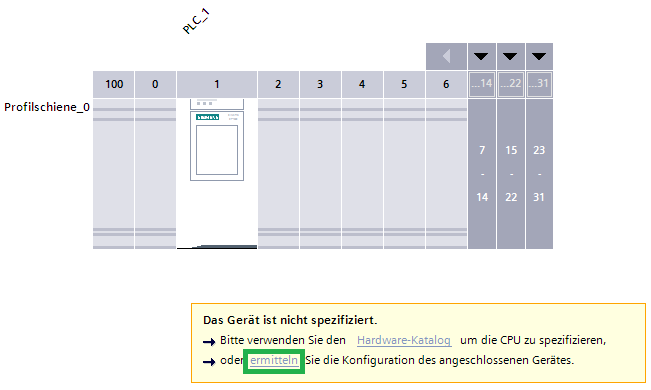
\includegraphics[width=0.7\textwidth]{Bilder/3. Konfiguration der S7-1500/3.2 Kommunikation herstellen/(3.2.1) Hardware ermitteln.png}}
   \caption[Hardware ermitteln]{Hardware ermitteln}
   \label{fig:Bild3.3}
\end{figure}

Einstellungen der Schnittstelle vornehmen und mit \glqq\textbf{Suche starten}\grqq\:nach Geräten suchen. Anschließend das richtige Gerät anhand der IP-Adresse (hier: 192.168.1.116) auswählen und mit \glqq\textbf{Erkennen}\grqq\:bestätigen.
\begin{figure}[H]
   \centering
   \fbox{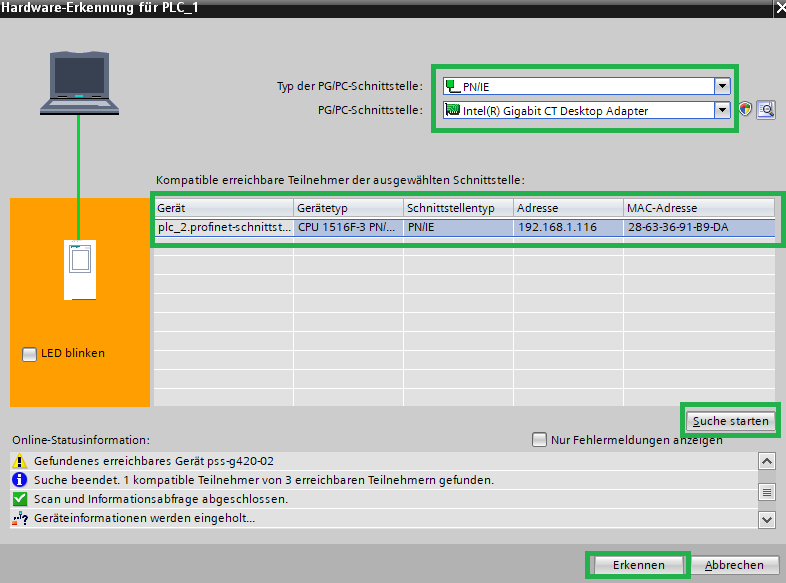
\includegraphics[width=0.6\textwidth]{Bilder/3. Konfiguration der S7-1500/3.2 Kommunikation herstellen/(3.2.2) Kommunikation aufnehmen.png}}
   \caption[Kommunikation herstellen]{Kommunikation herstellen}
   \label{fig:Bild3.4}
\end{figure}

Da das Gerät erstmalig hinzugefügt wurde, ist es sinnvoll, dies als vertrauenswürdig einzustufen (\autoref{fig:Bild3.5}). Die gemachten Einstellungen sollen nicht als Voreinstellungen übernommen werden (\autoref{fig:Bild3.6}).  
\begin{figure}[H]
   \centering
   \fbox{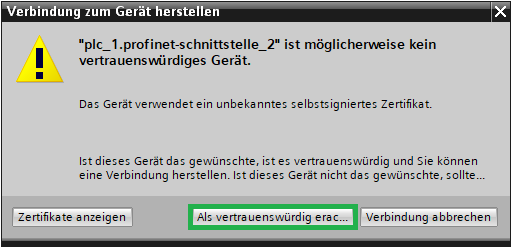
\includegraphics[width=0.75\textwidth]{Bilder/3. Konfiguration der S7-1500/3.2 Kommunikation herstellen/(3.2.3) Vertrauenswuerdigkeit zulassen.PNG}}
   \caption[Gerät als vertrauenswürdig einstufen]{Gerät als vertrauenswürdig einstufen}
   \label{fig:Bild3.5}
\end{figure}

\begin{figure}[H]
   \centering
   \fbox{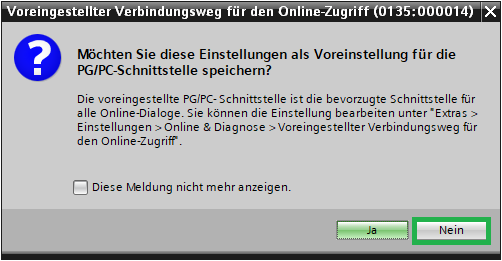
\includegraphics[width=0.75\textwidth]{Bilder/3. Konfiguration der S7-1500/3.2 Kommunikation herstellen/(3.2.4) Voreinstellungen nicht zulassen.PNG}}
   \caption[Nicht als Vorteinstellung übernehmen]{Nicht als Voreinstellung übernehmen}
   \label{fig:Bild3.6}
\end{figure}

\clearpage

\subsubsection{Security-Einstellungen der S7-1500}
Nachdem das Gerät erkannt wurde, öffnet sich das Fenster \textbf{PLC Security-Einstellungen}.\\
\textbf{ACHTUNG}: Dies hängt von der Version der S7-1500 ab.\\
\newline
1. Schutz vertraulicher PLC-Konfigurationsdaten \textbf{deaktivieren}:
\begin{figure}[H]
   \centering
   \fbox{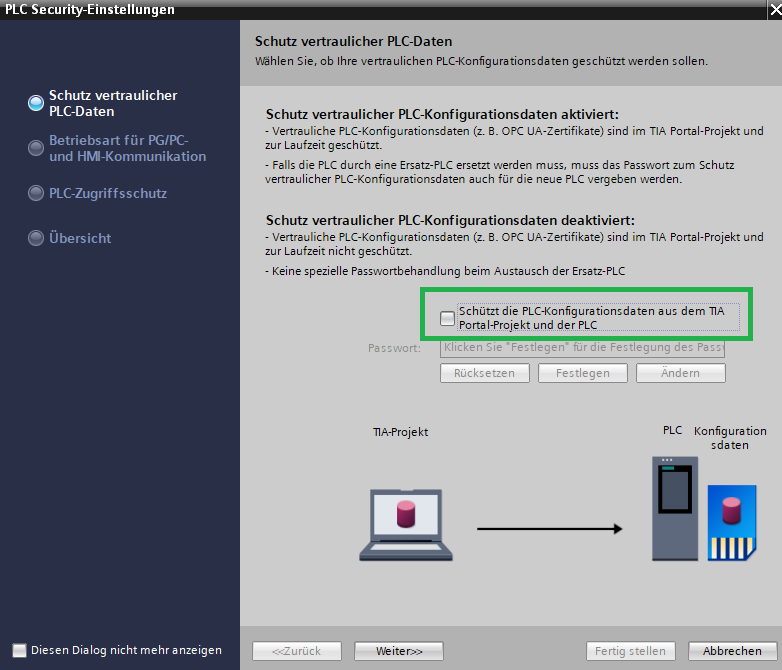
\includegraphics[width=0.8\textwidth]{Bilder/3. Konfiguration der S7-1500/3.3 Security-Einstellungen der S7-1500/(3.3.1) Security Einstellungen (1).png}}
   \caption[Security Einstellungen Teil 1]{Security Einstellungen Teil 1}
   \label{fig:Bild3.7}
\end{figure}

\clearpage

2. Legacy- und Secure PG/PC-Kommunikation \textbf{nicht zulassen}:
\begin{figure}[H]
   \centering
   \fbox{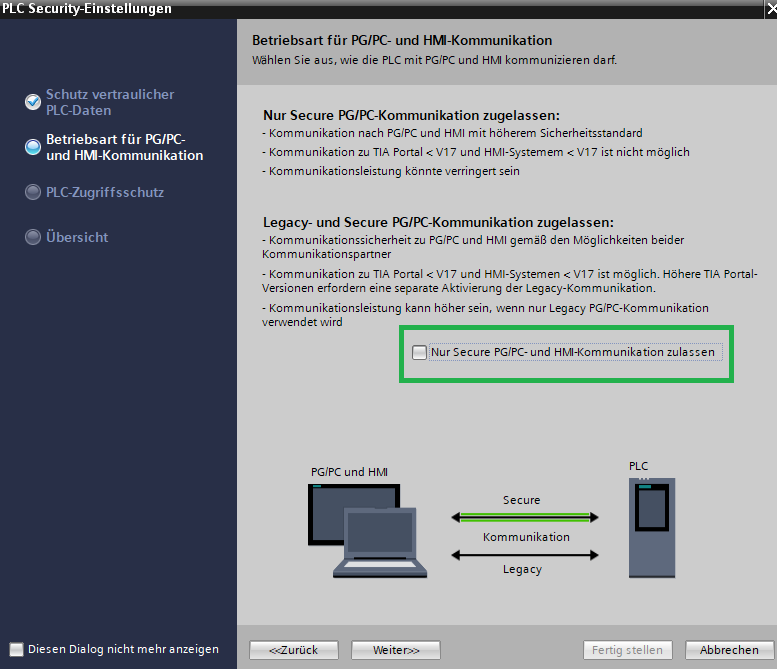
\includegraphics[width=0.8\textwidth]{Bilder/3. Konfiguration der S7-1500/3.3 Security-Einstellungen der S7-1500/(3.3.2) Security Einstellungen (2).png}}
   \caption[Security Einstellungen Teil 2]{Security Einstellungen Teil 2}
   \label{fig:Bild3.8}
\end{figure}

\clearpage

3. Zugriffstufe ohne Passwort auf \textbf{Vollzugriff inkl. fehlersicher (kein Schutz)} stellen:
\begin{figure}[H]
   \centering
   \fbox{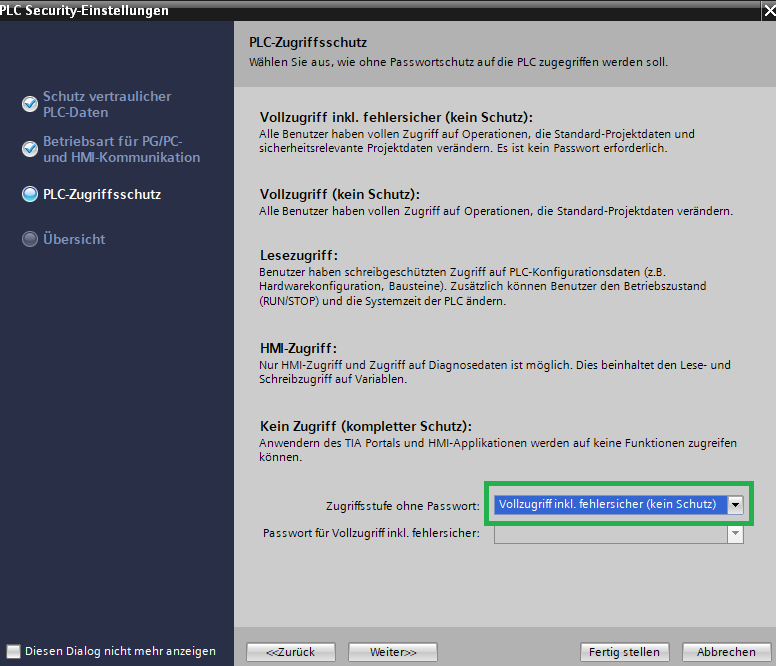
\includegraphics[width=0.8\textwidth]{Bilder/3. Konfiguration der S7-1500/3.3 Security-Einstellungen der S7-1500/(3.3.3) Security Einstellungen (3).png}}
   \caption[Security Einstellungen Teil 3]{Security Einstellungen Teil 3}
   \label{fig:Bild3.9}
\end{figure}

Die Einstellungen mit \glqq\textbf{Fertig stellen}\grqq\:übernehmen. Zuletzt über die \textbf{Gerätesicht} der S7-1500 den \textbf{Schreibzugriff deaktivieren}.\\
Pfad: Allgemein > Display > Passwort 
\begin{figure}[H]
   \centering
   \fbox{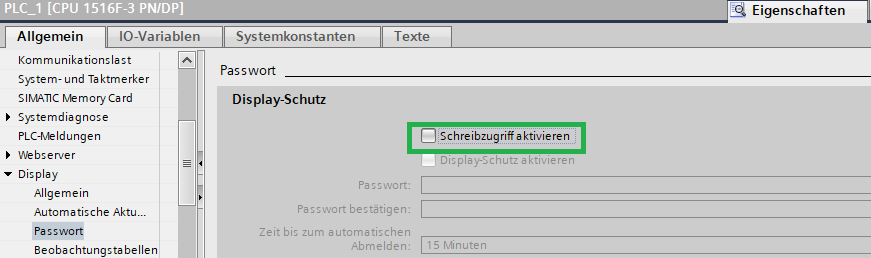
\includegraphics[width=0.8\textwidth]{Bilder/3. Konfiguration der S7-1500/3.3 Security-Einstellungen der S7-1500/(3.3.4) Passwortschutz entfernen.png}}
   \caption[Passwortschutz entfernen]{Passwortschutz entfernen}
   \label{fig:Bild3.10}
\end{figure}

\clearpage

\subsubsection{IP-Adresse und Vergabe des PROFINET-Gerätenamen der S7-1500} \label{sec: IP-Adresse_PROFINET-Gerätename_S7-1500}
Die jeweiligen IP-Adressen und PROFINET-Gerätenamen können der \autoref{fig:Bild1.3} entnommen werden. Die Bezeichnung des PROFINET-Anschlusses ist \textbf{X2}.

\begin{figure}[H]
   \centering
   \fbox{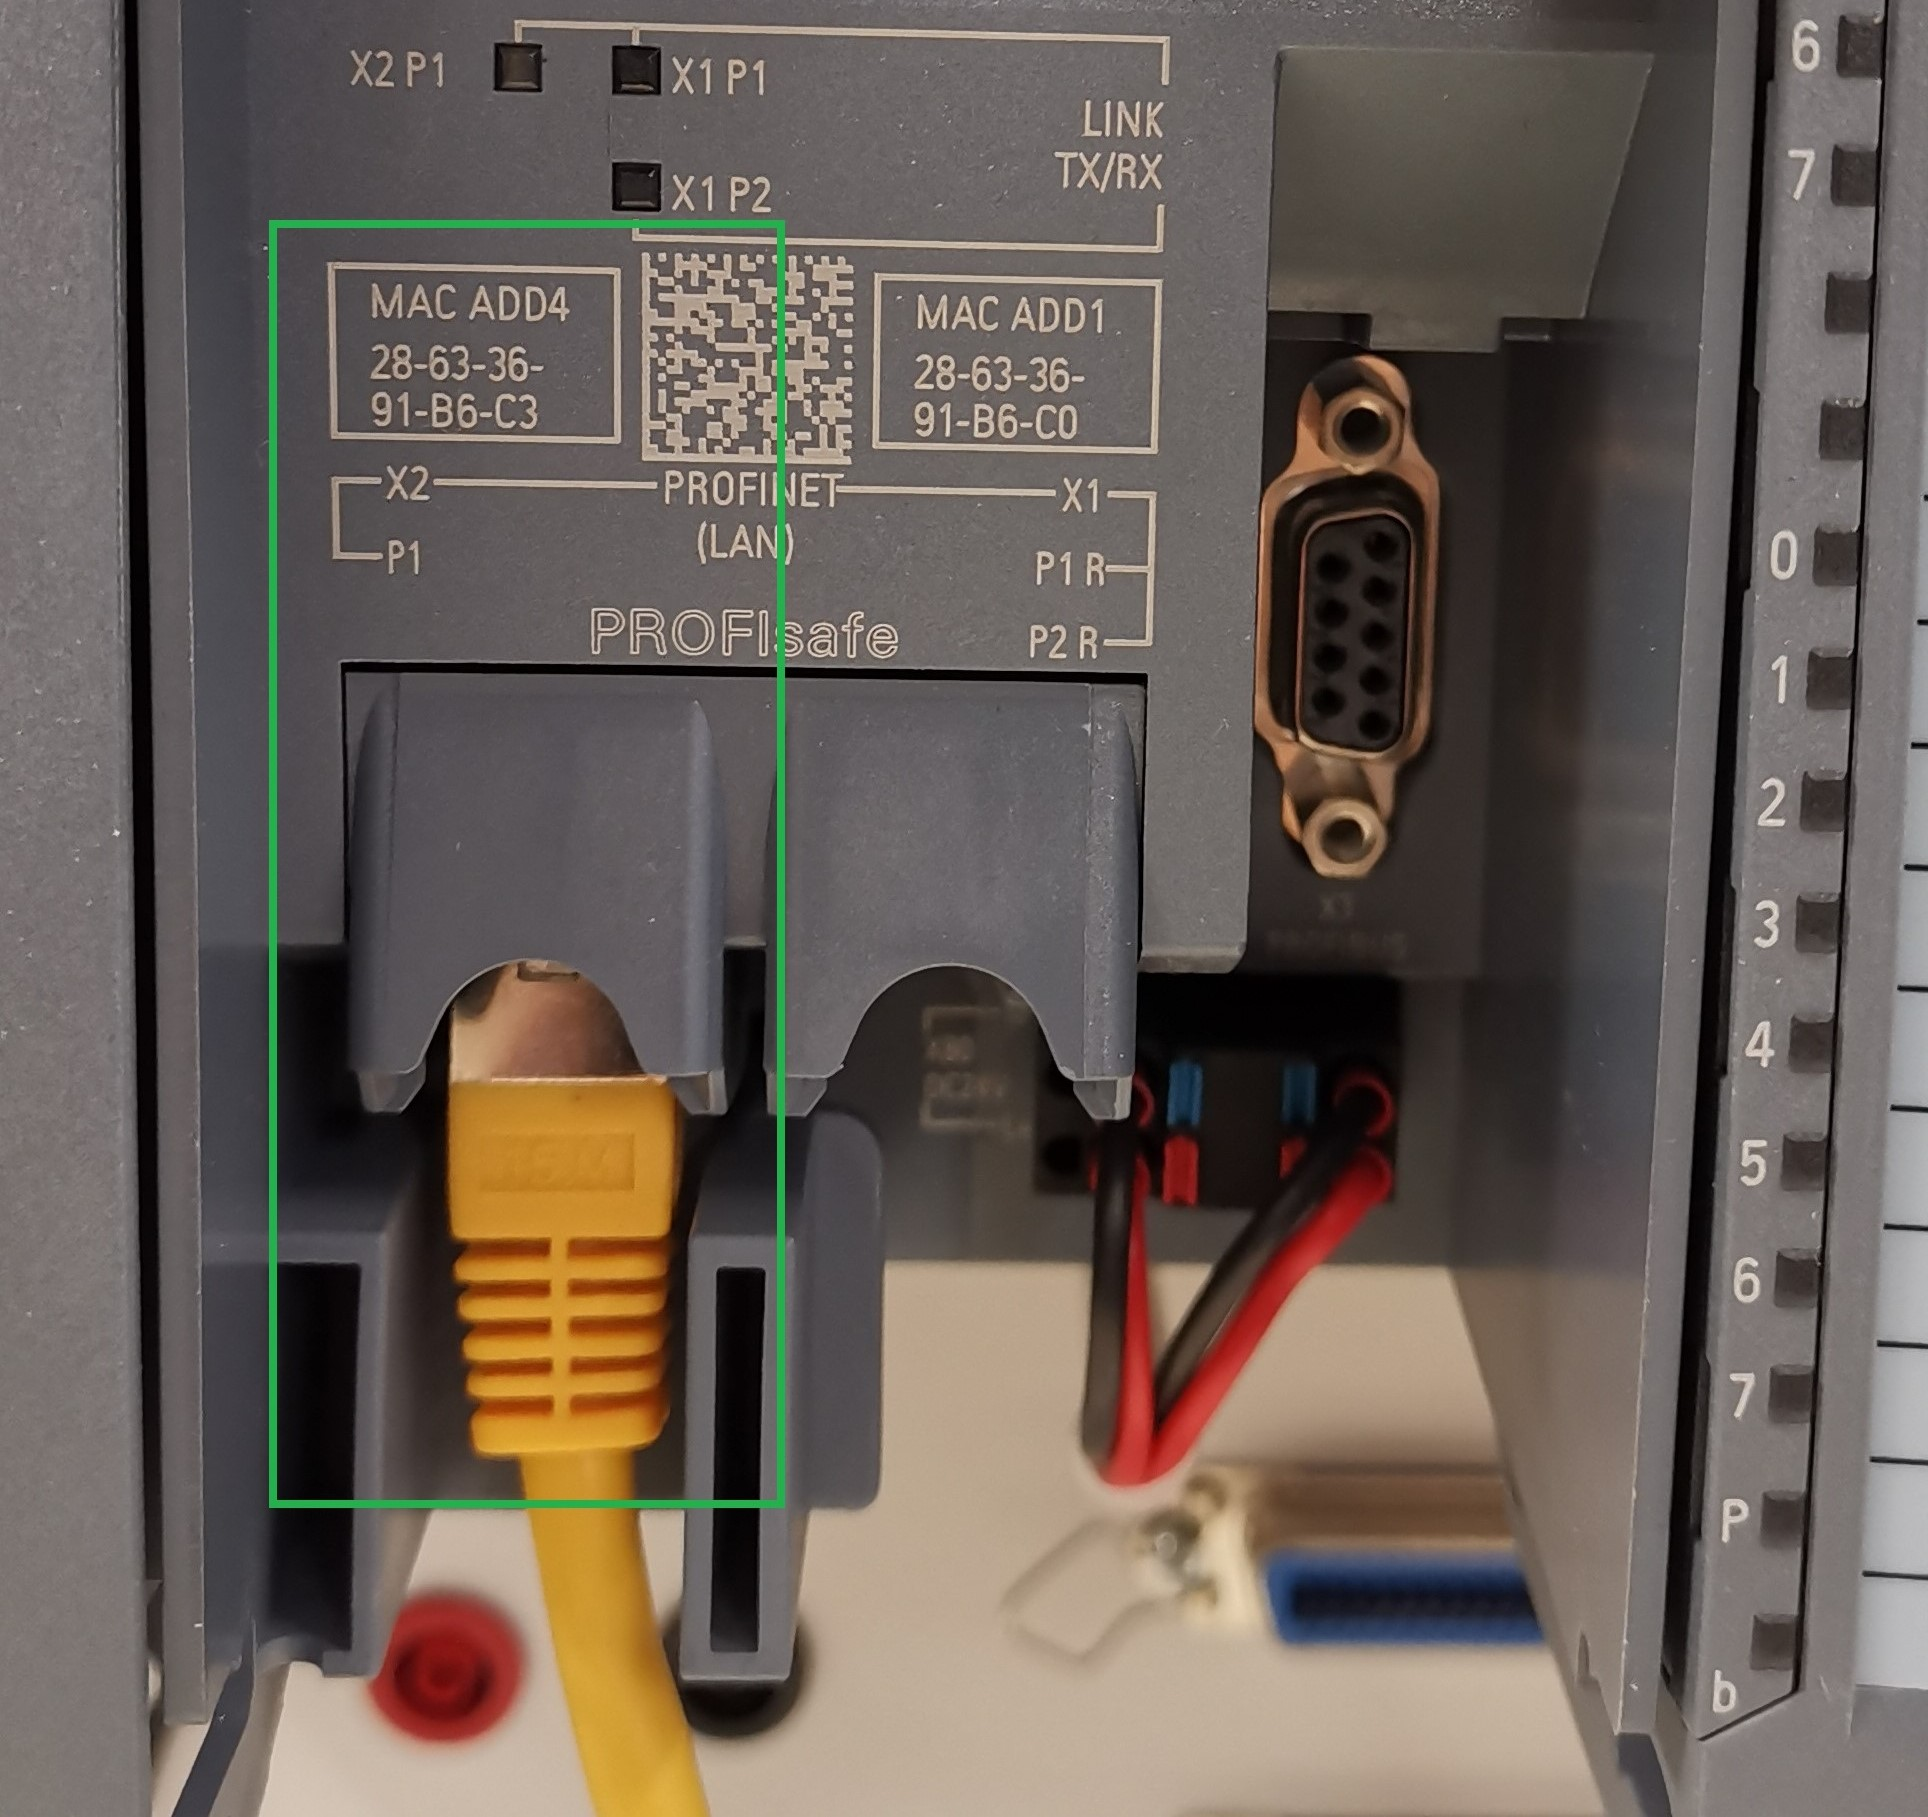
\includegraphics[width=0.45\textwidth]{Bilder/3. Konfiguration der S7-1500/3.4 IP-Adresse und Vergabe des PROFINET-Gerätenamen der S7-1500/(3.4.1) PROFINET-Schnittstelle.jpg}}
   \caption[Anschluss an PROFINET-Schnittstelle]{Anschluss an PROFINET-Schnittstelle}
   \label{fig:Bild3.11}
\end{figure}

1. IP-Adresse vergeben:\\
Pfad über \textbf{Gerätesicht}: Allgemein > PROFINET-Schnittstelle [X2] > Ethernet-Adressen
\begin{figure}[H]
   \centering
   \fbox{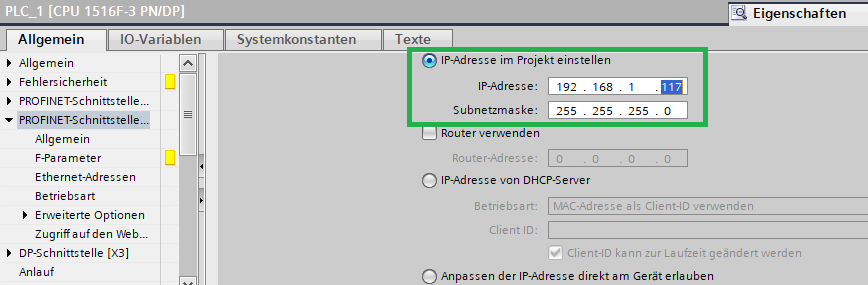
\includegraphics[width=0.9\textwidth]{Bilder/3. Konfiguration der S7-1500/3.4 IP-Adresse und Vergabe des PROFINET-Gerätenamen der S7-1500/(3.4.2) IP-Adresse der S7 einstellen.png}}
   \caption[IP-Adresse der S7-1500 eingeben]{IP-Adresse der S7-1500 eingeben}
   \label{fig:Bild3.12}
\end{figure}

\clearpage

2. PROFINET-Gerätename vergeben:\\
Pfad über \textbf{Gerätesicht}: Allgemein > PROFINET-Schnittstelle [X2] > Ethernet-Adressen\\
\newline
Zur Eingabe des PROFINET-Gerätenamen das Häkchen bei \glqq\textbf{PROFINET-Gerätename automatisch generieren}\grqq\:entfernen.

\begin{figure}[H]
   \centering
   \fbox{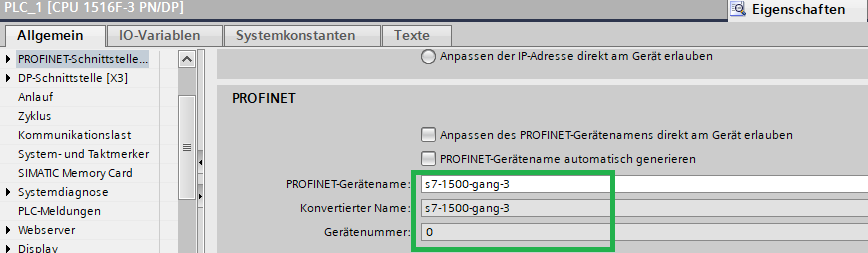
\includegraphics[width=0.9\textwidth]{Bilder/3. Konfiguration der S7-1500/3.4 IP-Adresse und Vergabe des PROFINET-Gerätenamen der S7-1500/(3.4.3) PROFINET-Geraetename S7 einstellen.png}}
   \caption[PROFINET-Gerätename der S7-1500 eingeben]{PROFINET-Gerätename der S7-1500 eingeben}
   \label{fig:Bild3.13}
\end{figure}

\subsection{Konfiguration der ET 200SP} \label{sec:Konfiguration_der_ET_200_SP}

\subsubsection{ET 200SP hinzufügen}
Über die \textbf{Netzsicht} im Katalog nach der Bezeichnung des \textbf{IM 155-Interfacemoduls} suchen (hier: IM 155-6PN HF (6ES7155-6AU00-0CN0)) und hinzufügen.\\
Pfad: Katalog > Dezentrale Peripherie > ET 200SP > Interfacemodule > PROFINET > IM 155-6 PN HF

\begin{figure}[H]
    \centering
   \begin{minipage}[b]{.4\linewidth}
        \centering
        \fbox{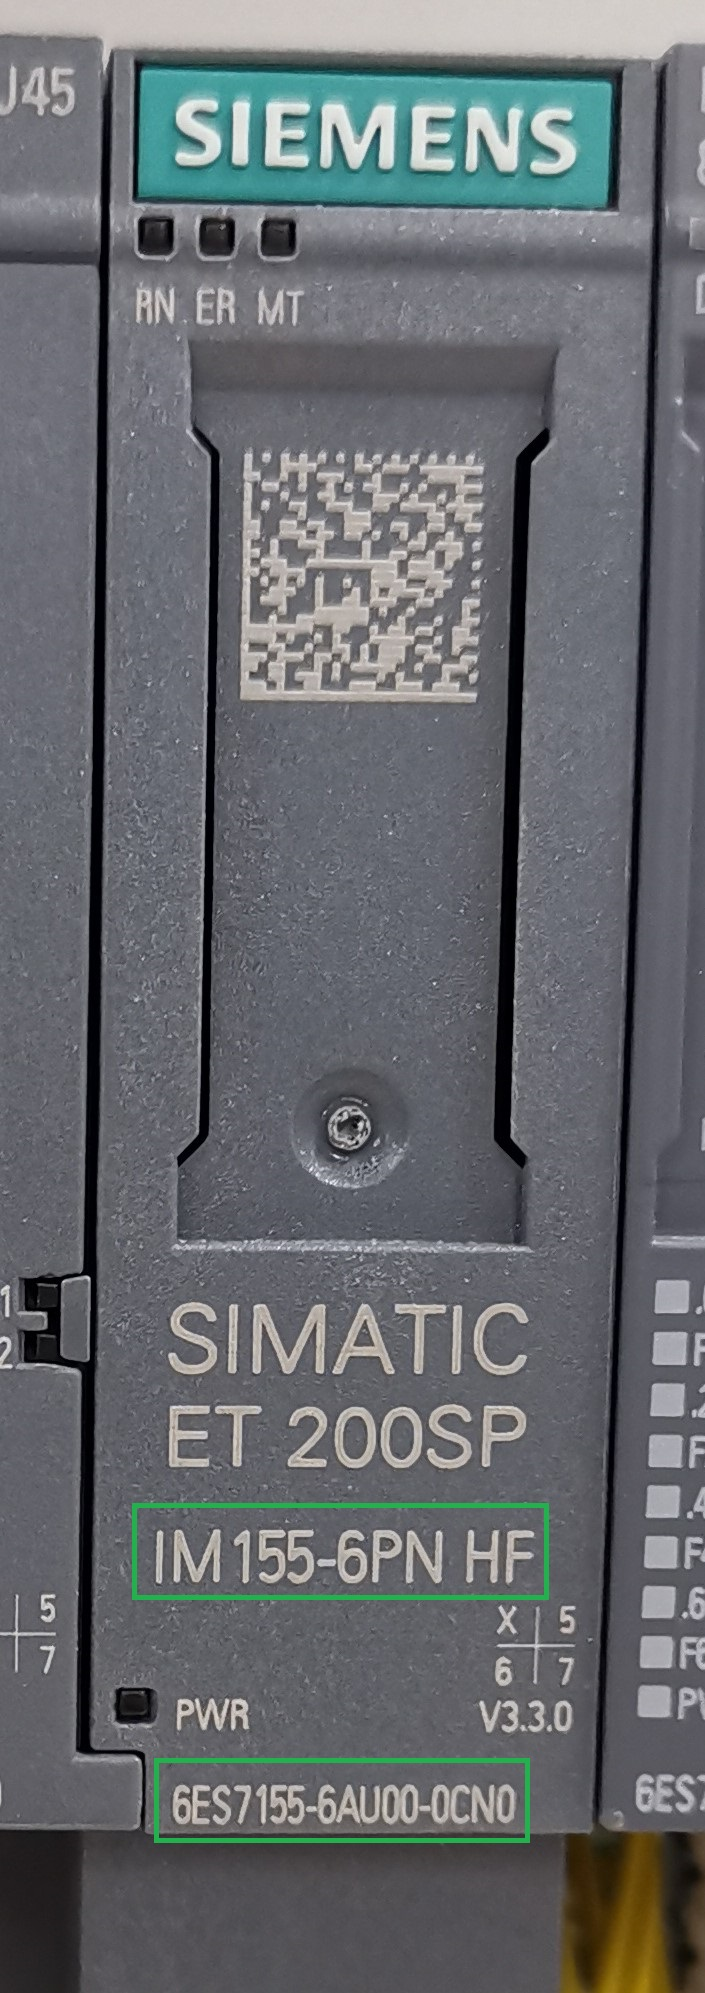
\includegraphics[width=0.4\linewidth]{Bilder/4. Konfiguration der ET 200 SP/4.1 ET 200 SP hinzufügen/(4.1.1) Modulbezeichnung am Beispiel des IM 155-Moduls.jpg}}
        \caption[Modulbezeichnung am Beispiel des IM 155-Interfacemoduls]{Modulbezeichnung am Beispiel des IM 155-Interfacemoduls}
        \label{fig:Bild4.1}
   \end{minipage}
   \hspace{.1\linewidth}% Abstand zwischen Bilder
   \begin{minipage}[b]{.4\linewidth}
        \centering
        \fbox{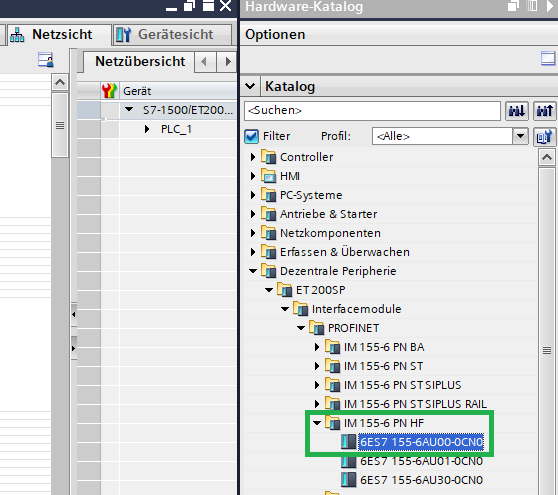
\includegraphics[width=1.1\linewidth]{Bilder/4. Konfiguration der ET 200 SP/4.1 ET 200 SP hinzufügen/(4.1.2) Dezentrale Peripherie hinzufuegen.png}}
        \caption[Dezentrale Peripherie hinzufügen]{Dezentrale Peripherie hinzufügen\\}
        \label{fig:Bild4.2}
   \end{minipage}
\end{figure}

\clearpage

\subsubsection{Module hinzufügen}
In der \textbf{Gerätesicht} der ET 200SP über den Katalog die weiteren Module hinzufügen.\\
\textbf{ACHTUNG:} Die Bezeichnungen auf den realen Modulen weichen teils von denen im TIA-Portal ab.

\begin{figure}[H]
   \centering
   \fbox{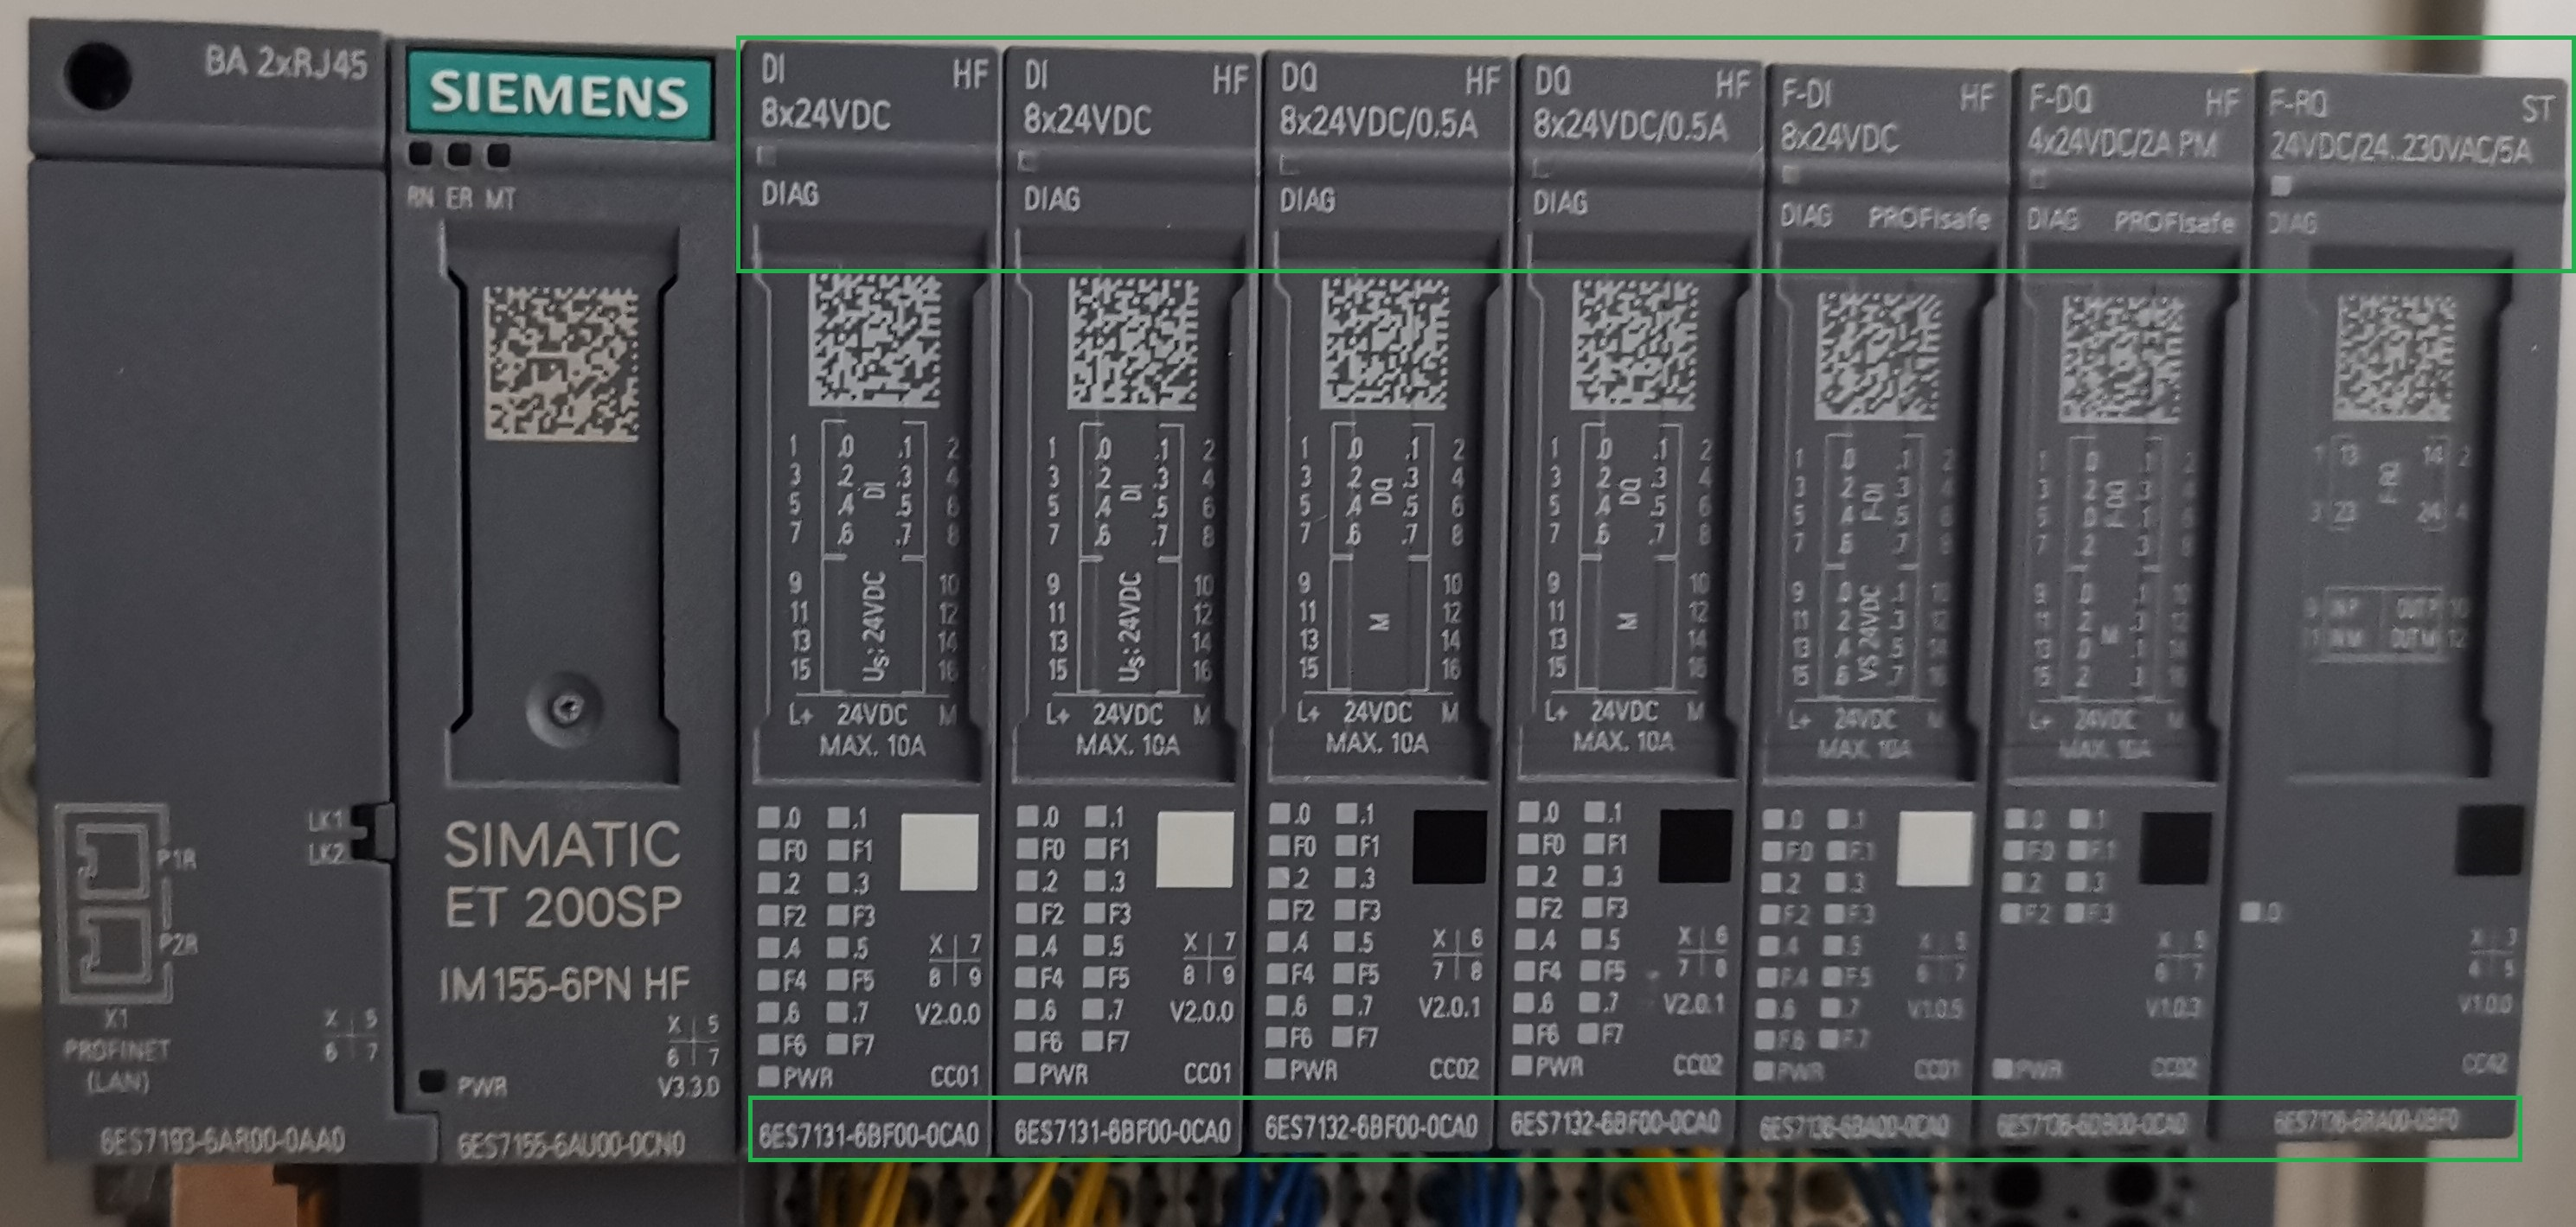
\includegraphics[width=0.9\textwidth]{Bilder/4. Konfiguration der ET 200 SP/4.2 Module hinzufügen/(4.2.1) Übersicht aller Module der dezentralen Peripherie.jpg}}
   \caption[Übersicht der Module der dezentralen Peripherie]{Übersicht der Module der dezentralen Peripherie}
   \label{fig:Bild4.3}
\end{figure}

\begin{table}[H]
    \centering
    \begin{tabular}{|c|c|c|}
        \hline
         \textbf{Modulbezeichnung} & \textbf{Modulnummer} & \textbf{Version} \\
         \hline
         DI 8x24VDC HF	& 6ES7131-6BF00-0CA0	& 2.0.0 \\
         \hline
         DI 8x24VDC HF	& 6ES7131-6BF00-0CA0	& 2.0.0 \\
         \hline
         DQ 8x24VDC/0.5A HF &	6ES7132-6BF00-0CA0	& 2.0.1 \\
         \hline
         DQ 8x24VDC/0.5A HF &	6ES7132-6BF00-0CA0	& 2.0.1 \\
         \hline
         F-DI 8x24VDC HF & 	6ES7136-6BA00-0CA0	& 1.0.5 \\
         \hline
         F-DQ 4x24VDC/2A PM HF & 	6ES7136-6DB00-0CA0	& 1.0.3 \\
         \hline
         F-RQ 24VDC/24…230VAC/5A ST & 	6ES7136-6RA00-09F0	& 1.0.0 \\
         \hline
    \end{tabular}
    \caption{Modulbezeichnungen, -nummern und -versionen}
    \label{tab:Tab4.1}
\end{table}

\begin{figure}[H]
   \centering
   \fbox{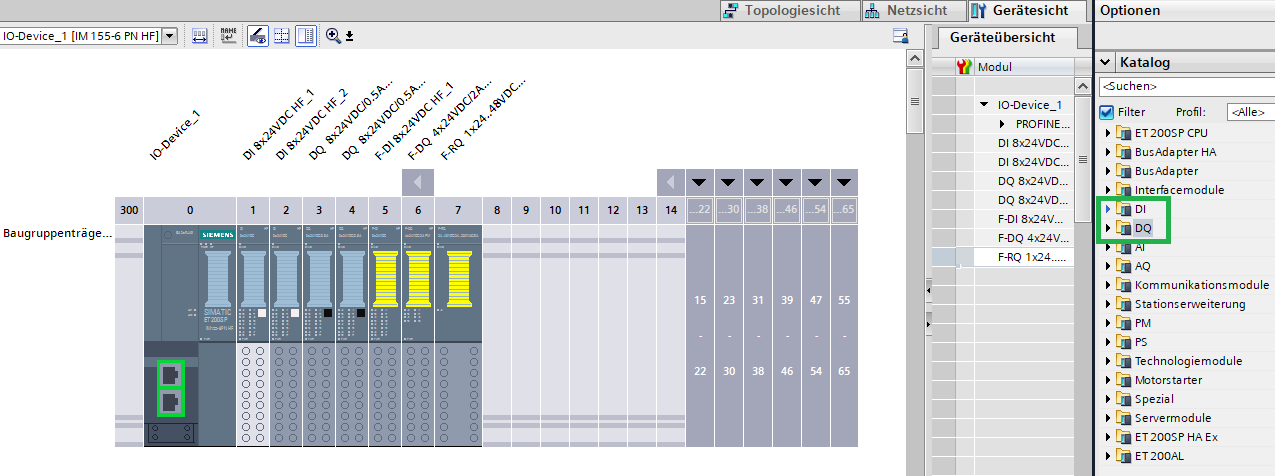
\includegraphics[width=0.9\textwidth]{Bilder/4. Konfiguration der ET 200 SP/4.2 Module hinzufügen/(4.2.2) Elemente der dezentralen Peripherie hinzufuegen.png}}
   \caption[Module hinzufügen]{Module hinzufügen}
   \label{fig:Bild4.4}
\end{figure}

Alle eingefügten Module (bis auf: F-RQ 24VDC/24…230VAC/5A ST) werden zu einer \textbf{Potentialgruppe} hinzugefügt. Dies kann durch das Anklicken der Module und dem anschließenden auswählen von \glqq\textbf{Neue Potentialgruppe ermöglichen (helle BaseUnit)}\grqq\:erfolgen.\\
Pfad: Allgemein > Potentialgruppe

\begin{figure}[H]
   \centering
   \fbox{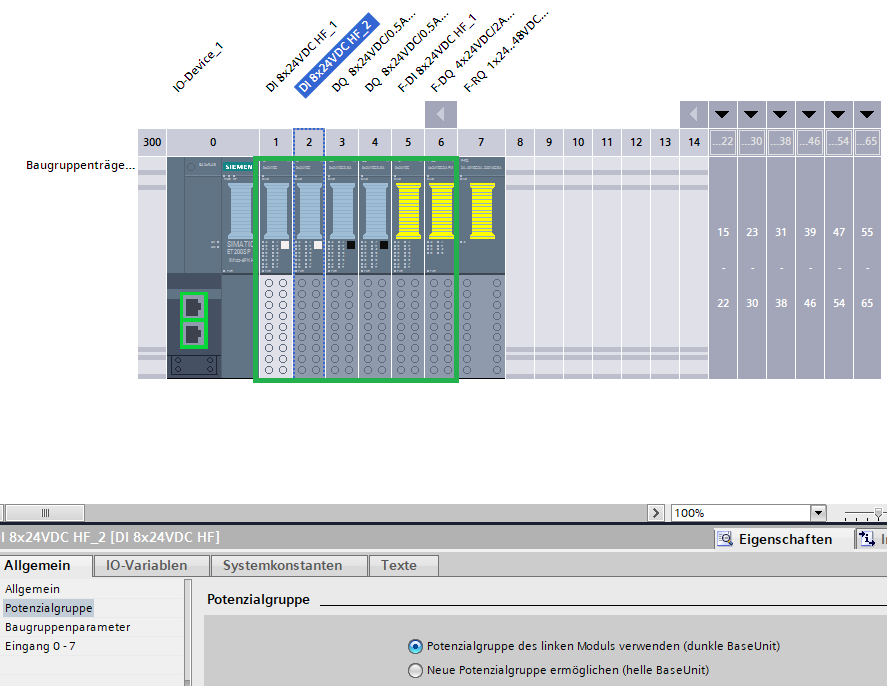
\includegraphics[width=0.75\textwidth]{Bilder/4. Konfiguration der ET 200 SP/4.2 Module hinzufügen/(4.2.3) Potenzialgruppe aendern.png}}
   \caption[Potenzialgruppe anpassen]{Potenzialgruppe anpassen}
   \label{fig:Bild4.5}
\end{figure}

\subsubsection{Geräteversionen tauschen}
Sofern dies nicht bereits beim Einfügen der Module beachtet wurde, müssen die Versionen des Interfacemoduls IM 155-6PN HF und des Moduls F-DQ angepasst werden. Dies kann durch einen Rechtsklick in der \textbf{Gerätesicht} auf das \glqq\textbf{Modul > Geräte tauschen..}\grqq\:durchgeführt werden. Die Versionsnummern siehe \autoref{tab:Tab4.1}. \\
\textbf{ACHTUNG:} Die Artikel-Nummern müssen übereinstimmen.

\begin{figure}[H]
   \centering
   \fbox{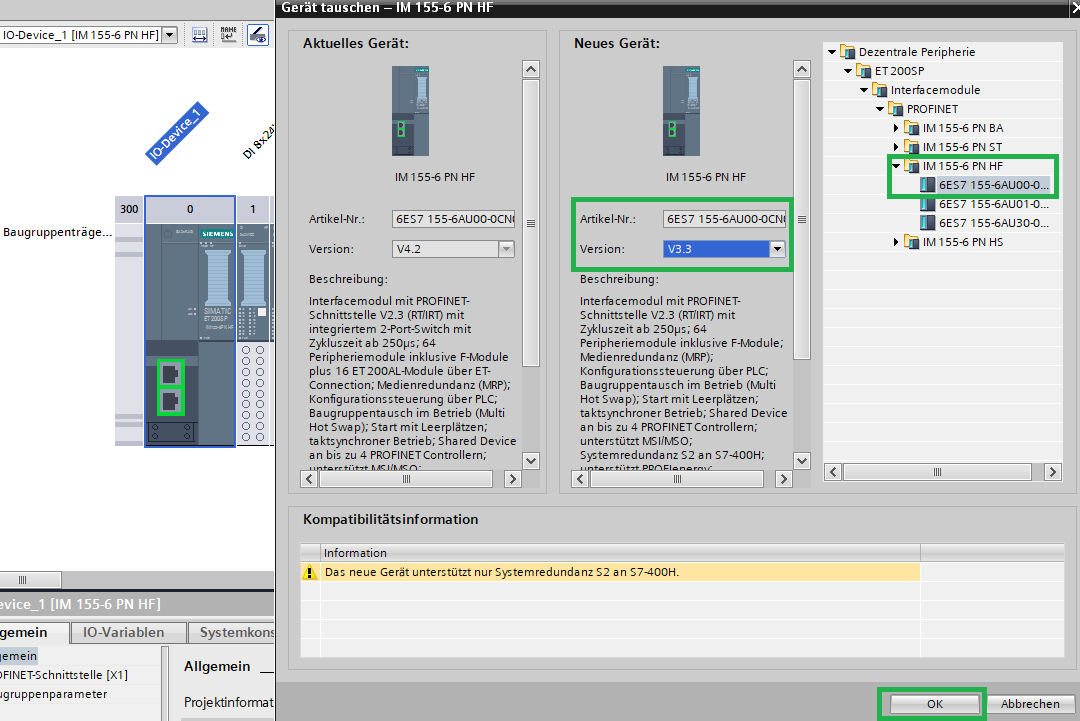
\includegraphics[width=0.65\textwidth]{Bilder/4. Konfiguration der ET 200 SP/4.3 Geräteversionen tauschen/(4.3.1) Geraeteversion tauschen.png}}
   \caption[Geräteversion des IM 155-Interfacemoduls tauschen]{Geräteversion des IM 155-Interfacemoduls tauschen}
   \label{fig:Bild4.6}
\end{figure}

\begin{figure}[H]
   \centering
   \fbox{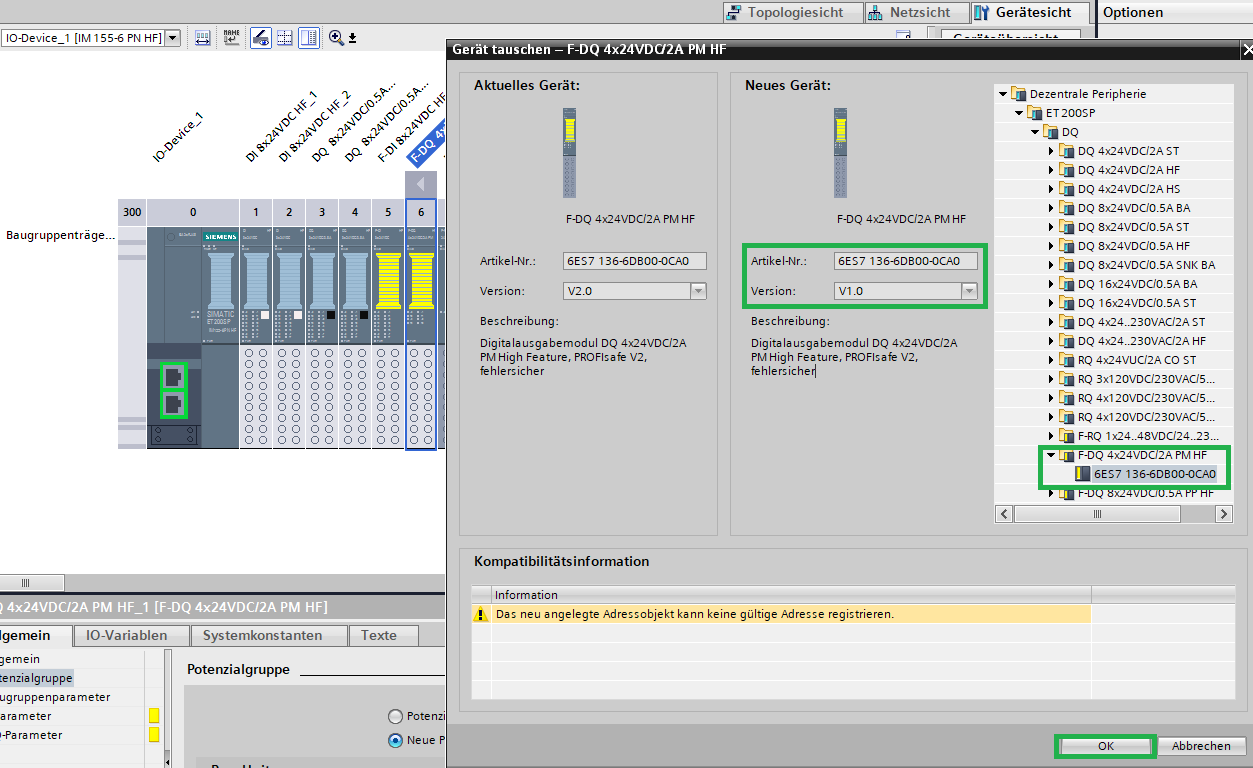
\includegraphics[width=0.65\textwidth]{Bilder/4. Konfiguration der ET 200 SP/4.3 Geräteversionen tauschen/(4.3.2) Geraeteversion tauschen.png}}
   \caption[Geräteversion des F-DQ-Moduls tauschen]{Geräteversion des F-DQ-Moduls tauschen}
   \label{fig:Bild4.7}
\end{figure}

\subsubsection{IP-Adresse und Vergabe des PROFINET-Gerätenamen der ET 200SP} \label{sec: IP-Adresse_PROFINET-Gerätename_ET_200SP}
Die Bezeichnung der PROFINET-Schnittstelle der ET 200SP ist \textbf{X1}.

\begin{figure}[H]
   \centering
   \fbox{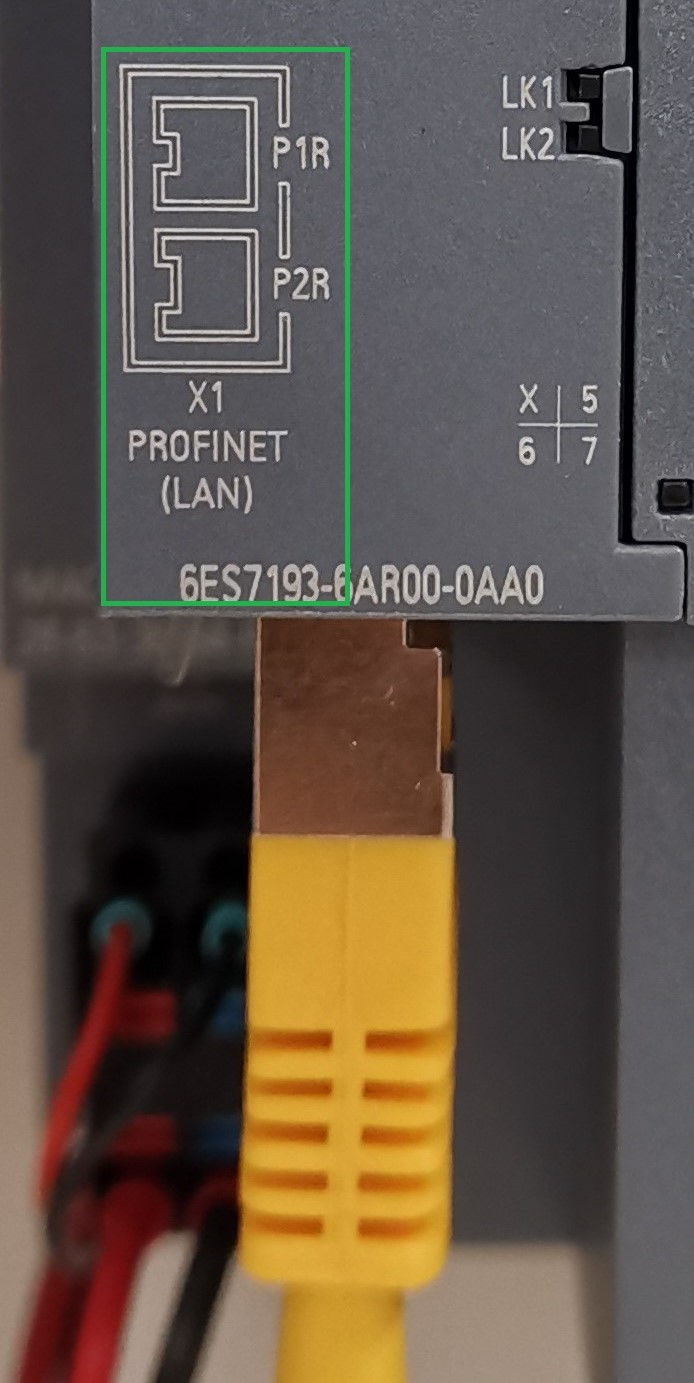
\includegraphics[width=0.2\textwidth]{Bilder/4. Konfiguration der ET 200 SP/4.4 IP-Adresse und Vergabe des PROFINET-Gerätenamen der ET 200 SP/(4.4.1) Bezeichnung der PROFINET-Schnittstelle.jpg}}
   \caption[Bezeichnung der PROFINET-Schnitstelle der ET 200SP]{Bezeichnung der PROFINET-Schnittstelle der ET 200SP}
   \label{fig:Bild4.8}
\end{figure}

Die benötigte IP-Adresse und PROFINET-Gerätename können der \autoref{fig:Bild1.3} entnommen werden. Die Einstellungen sind über die \textbf{Gerätesicht} des Gerätes ET 200SP sichtbar. Bei der Vergabe des PROFINET-Gerätenamens das Häkchen bei \glqq\textbf{PROFINET-Gerätename automatisch generieren}\grqq\:entfernen.\\
Pfad: Allgemein > PROFINET-Schnittstelle [X1]

\begin{figure}[H]
   \centering
   \fbox{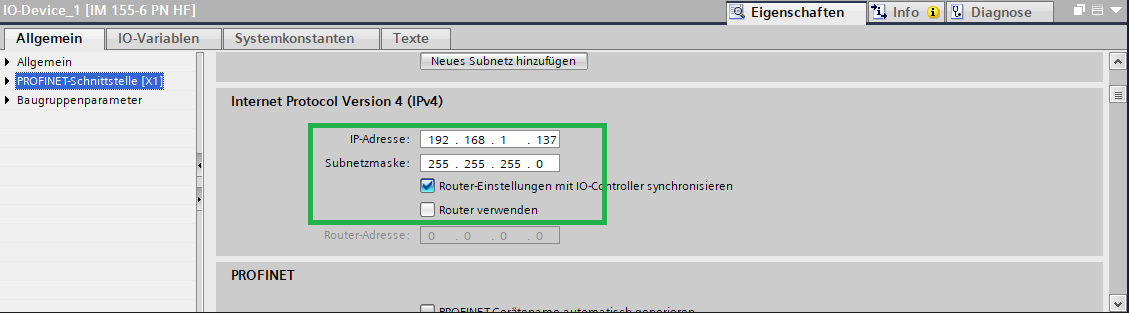
\includegraphics[width=1\textwidth]{Bilder/4. Konfiguration der ET 200 SP/4.4 IP-Adresse und Vergabe des PROFINET-Gerätenamen der ET 200 SP/(4.4.2) IP-Adresse der ET 200 SP.png}}
   \caption[Vergabe der IP-Adresse der ET 200SP]{Vergabe der IP-Adresse der ET 200SP}
   \label{fig:Bild4.9}
\end{figure}

\begin{figure}[H]
   \centering
   \fbox{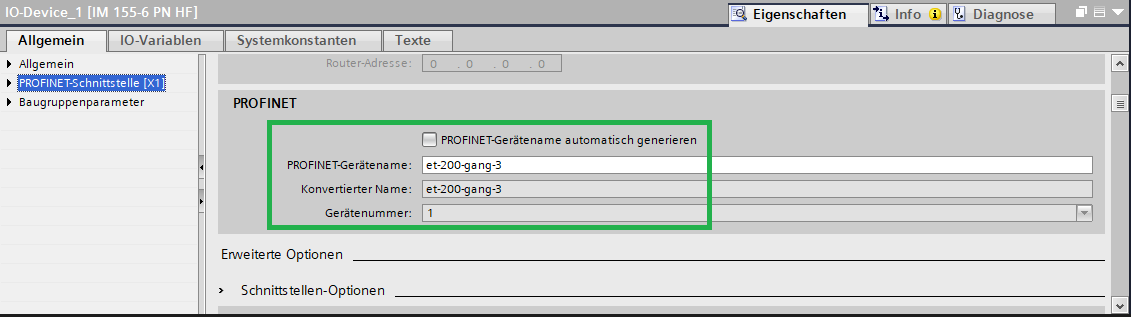
\includegraphics[width=1\textwidth]{Bilder/4. Konfiguration der ET 200 SP/4.4 IP-Adresse und Vergabe des PROFINET-Gerätenamen der ET 200 SP/(4.4.3) PROFINET-Geraetename der ET 200 SP.png}}
   \caption[Vergabe des PROFINET-Gerätenamen der ET 200SP]{Vergabe des PROFINET-Gerätenamen der ET 200SP}
   \label{fig:Bild4.10}
\end{figure}

\subsection{PROFINET-Verbindung} \label{sec:ergebnisse}

\subsubsection{Verbindung herstellen} \label{sec: Verbindung herstellen}
Die PROFINET-Verbindung beider Geräte und deren Module wird über die \textbf{Netzsicht} vorgenommen. Dabei ist auf die richtigen Anschlüssen zu achten (s. \autoref{sec: IP-Adresse_PROFINET-Gerätename_S7-1500} und \autoref{sec: IP-Adresse_PROFINET-Gerätename_ET_200SP}).

\begin{figure}[H]
   \centering
   \fbox{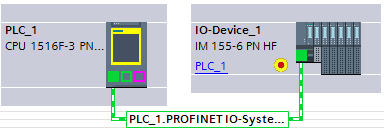
\includegraphics[width=0.8\textwidth]{Bilder/5. PROFINET-Verbindung/5.1 Verbindung herstellen/(5.1.1) PROFINET-Verbindung ziehen.png}}
   \caption[PROFINET-Verbindung herstellen]{PROFINET-Verbindung herstellen}
   \label{fig:Bild5.1}
\end{figure}

\subsubsection{Fehlersicherheit aktivieren}
Zusätzlich zur PROFINET-Verbindung in der Netzsicht ist in den Einstellungen der S7-1500 (über \textbf{Gerätesicht}) die Fehlersicherheit (\textbf{F-Fähigkeit}) zu aktivieren.\\
Pfad: Fehlersicherheit > F-Aktivierung

\begin{figure}[H]
   \centering
   \fbox{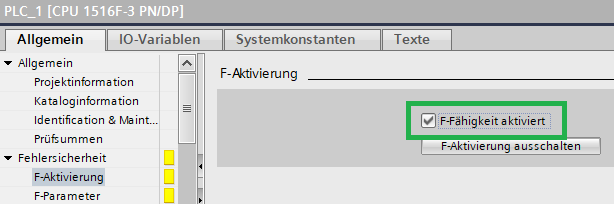
\includegraphics[width=0.8\textwidth]{Bilder/5. PROFINET-Verbindung/5.2 Fehlersicherheit aktivieren/(5.2.1) Fehlersicherheit aktivieren.png}}
   \caption[Fehlersicherheit aktivieren]{Fehlersicherheit aktivieren}
   \label{fig:Bild5.2}
\end{figure}

\subsubsection{Überprüfung des internen PROFINET-Gerätenamens der ET 200SP}
Möglicherweise stimmt der intern festgelegte Gerätename nicht mit dem nach \autoref{sec: IP-Adresse_PROFINET-Gerätename_ET_200SP} vergebenen überein. Um dies zu kontrollieren, kann über einen Rechtsklick auf die gesetzte PROFINET-Verbindung in der Netzsicht (s. \autoref{sec: Verbindung herstellen}) der Gerätename der ET 200SP ausgelesen und abgeglichen werden (\textbf{Rechtsklick > Gerätename zuweisen}).(\autoref{fig:Bild3.5}).  Stimmen die Gerätenamen nicht überein, muss der Name entsprechend geändert werden (s. \autoref{sec: IP-Adresse_PROFINET-Gerätename_ET_200SP}).

\begin{figure}[H]
   \centering
   \fbox{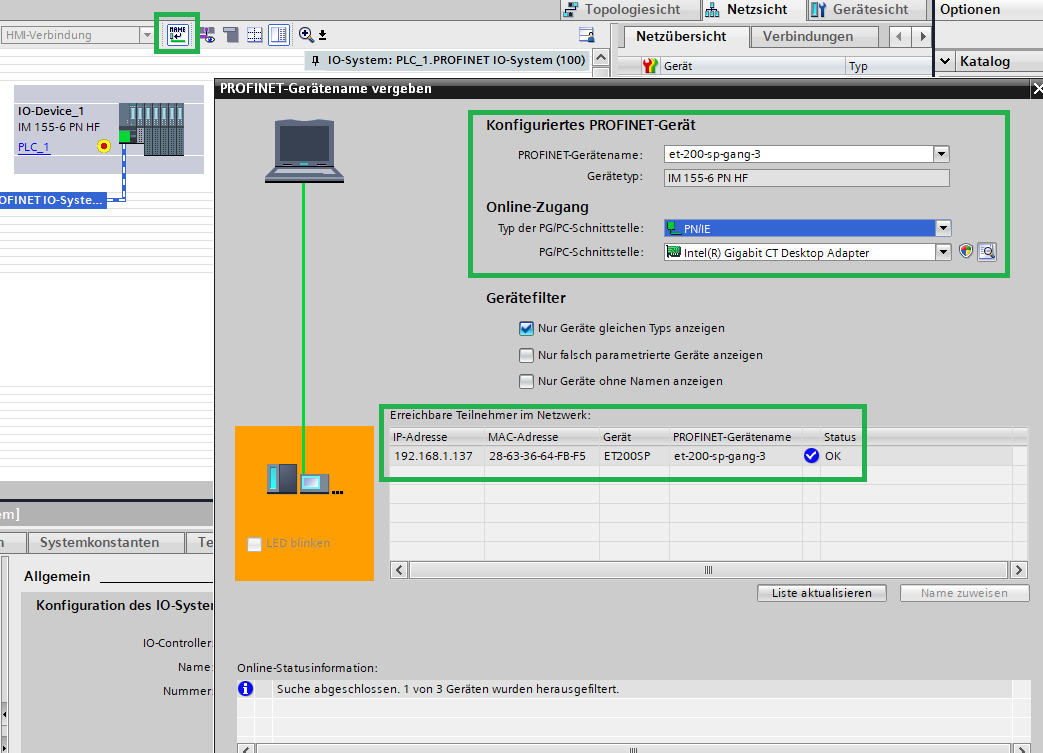
\includegraphics[width=0.8\textwidth]{Bilder/5. PROFINET-Verbindung/5.3 Überprüfung des internen PROFINET-Gerätenamens der ET 200SP/(5.3.1) Ueberpruefung der richtigen Namen.png}}
   \caption[Überprüfung des internen Gerätenamens der ET 200SP]{Überprüfung des internen Gerätenamens der ET 200SP}
   \label{fig:Bild5.3}
\end{figure}

\subsubsection{Überprüfung der IP-Adressen der Geräte}
Eine weitere Überprüfung für die korrekte Verbindung ist in der Netzsicht über den Button \glqq\textbf{Adressen anzeigen}\grqq\:möglich. Hierbei werden die IP-Adressen der Geräte angezeigt. Diese können mit der \autoref{fig:Bild1.3} abgeglichen werden. Sofern keine Verbindung hergestellt wurde, wird eine Fehlermeldung ausgegeben.

\begin{figure}[H]
   \centering
   \fbox{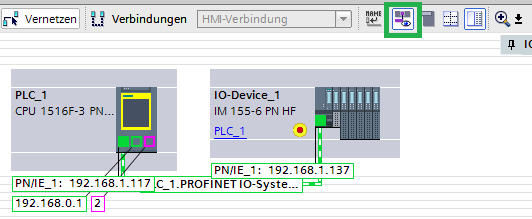
\includegraphics[width=0.8\textwidth]{Bilder/5. PROFINET-Verbindung/5.4 Überprüfung der IP-Adressen der Geräte/(5.4.1) Ueberpruefung der richtigen Adressen.png}}
   \caption[Überprüfung der IP-Adressen der Geräte]{Überprüfung der IP-Adressen der Geräte}
   \label{fig:Bild5.4}
\end{figure}

\subsection{Laden und Übersetzen der Hard- und Software} \label{sec: laden_und_uebersetzen}

Bevor eine Online-Verbindung mit der SPS aufgebaut werden kann, wird die Hard- und Software übersetzt (\autoref{fig:Bild6.1}) und anschließend in das Gerät geladen (\autoref{fig:Bild6.2}).

\begin{figure}[H]
   \centering
   \fbox{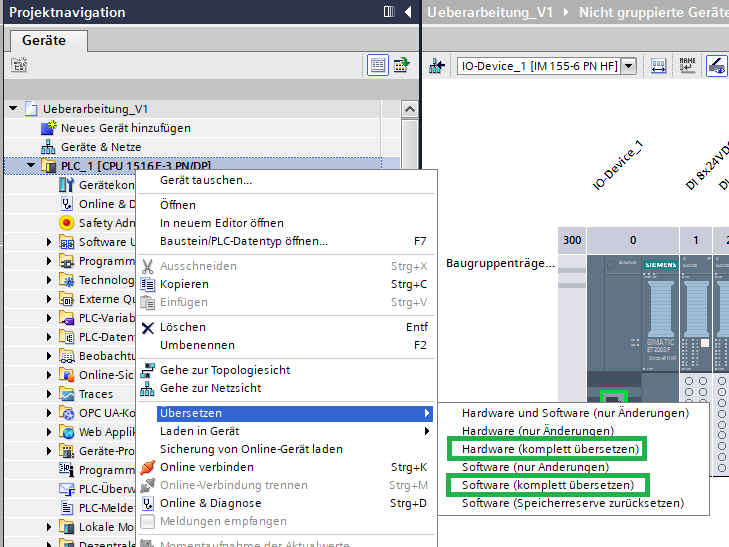
\includegraphics[width=0.6\textwidth]{Bilder/6. Laden und Übersetzen der Hard- und Software/(6.1) Uebersetzen.PNG}}
   \caption[Übersetzen der Hard- und Software]{Übersetzen der Hard- und Software}
   \label{fig:Bild6.1}
\end{figure}

\begin{figure}[H]
   \centering
   \fbox{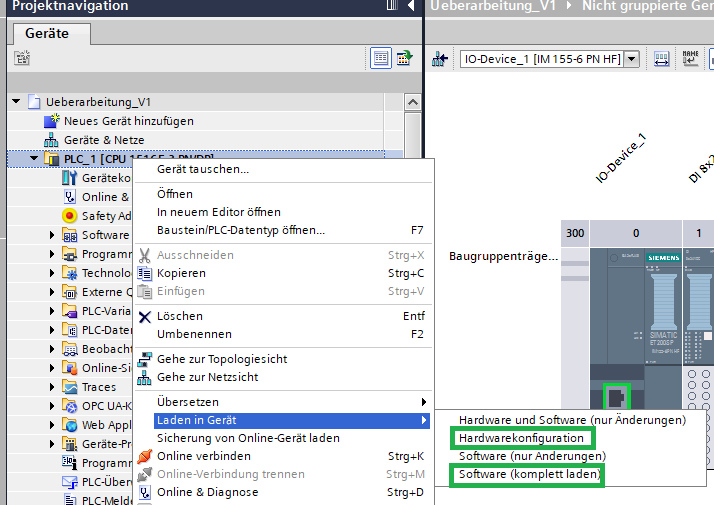
\includegraphics[width=0.6\textwidth]{Bilder/6. Laden und Übersetzen der Hard- und Software/(6.2) Laden.PNG}}
   \caption[Laden der Hard- und Software]{Laden der Hard- und Software}
   \label{fig:Bild6.2}
\end{figure}

\subsection{Vergabe der PROFIsafe-Adressen} \label{sec: vergabe der profisafe-adressen}

Nachdem die Online-Verbindung über \glqq\textbf{Online verbinden}\grqq\:hergestellt wurde, müssen die PROFIsafe-Adressen der F-DI und der F-DQ-Module vergeben werden. Dies kann durch einen \textbf{Rechtsklick auf Modul > PROFIsafe-Adresse zuweisen} durchgeführt werden. Anschließend wird das Menü aus \autoref{fig:Bild7.1} geöffnet. Nach Eingabe der Einstellungen des Online-Zugangs wird über \glqq\textbf{Identifikation}\grqq\:das entsprechende Modul ausgewählt. Durch das Setzen des Häkchen bei \glqq\textbf{Bestätigen}\grqq\:und dem Drücken von \glqq\textbf{PROFIsafe-Adresse zuweisen}\grqq\:wird die Einstellung übernommen.

\begin{figure}[H]
   \centering
   \fbox{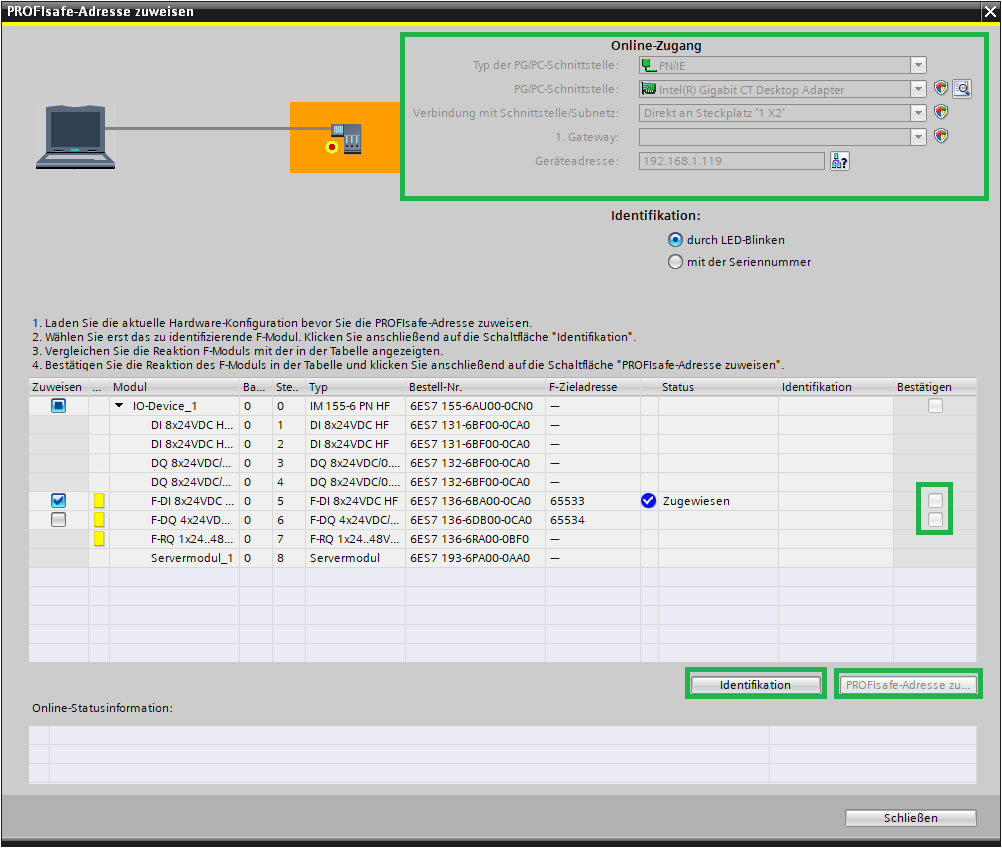
\includegraphics[width=1\textwidth]{Bilder/7. Vergabe der PROFIsafe-Adressen/(7.1) Vergabe der PROFIsafe-Adressen.PNG}}
   \caption[Vergabe der PROFIsafe-Adressen]{Vergabe der PROFIsafe-Adressen}
   \label{fig:Bild7.1}
\end{figure}
